\documentclass[1p]{elsarticle_modified}
%\bibliographystyle{elsarticle-num}

%\usepackage[colorlinks]{hyperref}
%\usepackage{abbrmath_seonhwa} %\Abb, \Ascr, \Acal ,\Abf, \Afrak
\usepackage{amsfonts}
\usepackage{amssymb}
\usepackage{amsmath}
\usepackage{amsthm}
\usepackage{scalefnt}
\usepackage{amsbsy}
\usepackage{kotex}
\usepackage{caption}
\usepackage{subfig}
\usepackage{color}
\usepackage{graphicx}
\usepackage{xcolor} %% white, black, red, green, blue, cyan, magenta, yellow
\usepackage{float}
\usepackage{setspace}
\usepackage{hyperref}

\usepackage{tikz}
\usetikzlibrary{arrows}

\usepackage{multirow}
\usepackage{array} % fixed length table
\usepackage{hhline}

%%%%%%%%%%%%%%%%%%%%%
\makeatletter
\renewcommand*\env@matrix[1][\arraystretch]{%
	\edef\arraystretch{#1}%
	\hskip -\arraycolsep
	\let\@ifnextchar\new@ifnextchar
	\array{*\c@MaxMatrixCols c}}
\makeatother %https://tex.stackexchange.com/questions/14071/how-can-i-increase-the-line-spacing-in-a-matrix
%%%%%%%%%%%%%%%

\usepackage[normalem]{ulem}

\newcommand{\msout}[1]{\ifmmode\text{\sout{\ensuremath{#1}}}\else\sout{#1}\fi}
%SOURCE: \msout is \stkout macro in https://tex.stackexchange.com/questions/20609/strikeout-in-math-mode

\newcommand{\cancel}[1]{
	\ifmmode
	{\color{red}\msout{#1}}
	\else
	{\color{red}\sout{#1}}
	\fi
}

\newcommand{\add}[1]{
	{\color{blue}\uwave{#1}}
}

\newcommand{\replace}[2]{
	\ifmmode
	{\color{red}\msout{#1}}{\color{blue}\uwave{#2}}
	\else
	{\color{red}\sout{#1}}{\color{blue}\uwave{#2}}
	\fi
}

\newcommand{\Sol}{\mathcal{S}} %segment
\newcommand{\D}{D} %diagram
\newcommand{\A}{\mathcal{A}} %arc


%%%%%%%%%%%%%%%%%%%%%%%%%%%%%5 test

\def\sl{\operatorname{\textup{SL}}(2,\Cbb)}
\def\psl{\operatorname{\textup{PSL}}(2,\Cbb)}
\def\quan{\mkern 1mu \triangleright \mkern 1mu}

\theoremstyle{definition}
\newtheorem{thm}{Theorem}[section]
\newtheorem{prop}[thm]{Proposition}
\newtheorem{lem}[thm]{Lemma}
\newtheorem{ques}[thm]{Question}
\newtheorem{cor}[thm]{Corollary}
\newtheorem{defn}[thm]{Definition}
\newtheorem{exam}[thm]{Example}
\newtheorem{rmk}[thm]{Remark}
\newtheorem{alg}[thm]{Algorithm}

\newcommand{\I}{\sqrt{-1}}
\begin{document}

%\begin{frontmatter}
%
%\title{Boundary parabolic representations of knots up to 8 crossings}
%
%%% Group authors per affiliation:
%\author{Yunhi Cho} 
%\address{Department of Mathematics, University of Seoul, Seoul, Korea}
%\ead{yhcho@uos.ac.kr}
%
%
%\author{Seonhwa Kim} %\fnref{s_kim}}
%\address{Center for Geometry and Physics, Institute for Basic Science, Pohang, 37673, Korea}
%\ead{ryeona17@ibs.re.kr}
%
%\author{Hyuk Kim}
%\address{Department of Mathematical Sciences, Seoul National University, Seoul 08826, Korea}
%\ead{hyukkim@snu.ac.kr}
%
%\author{Seokbeom Yoon}
%\address{Department of Mathematical Sciences, Seoul National University, Seoul, 08826,  Korea}
%\ead{sbyoon15@snu.ac.kr}
%
%\begin{abstract}
%We find all boundary parabolic representation of knots up to 8 crossings.
%
%\end{abstract}
%\begin{keyword}
%    \MSC[2010] 57M25 
%\end{keyword}
%
%\end{frontmatter}

%\linenumbers
%\tableofcontents
%
\newcommand\colored[1]{\textcolor{white}{\rule[-0.35ex]{0.8em}{1.4ex}}\kern-0.8em\color{red} #1}%
%\newcommand\colored[1]{\textcolor{white}{ #1}\kern-2.17ex	\textcolor{white}{ #1}\kern-1.81ex	\textcolor{white}{ #1}\kern-2.15ex\color{red}#1	}

{\Large $\underline{12a_{1206}~(K12a_{1206})}$}

\setlength{\tabcolsep}{10pt}
\renewcommand{\arraystretch}{1.6}
\vspace{1cm}\begin{tabular}{m{100pt}>{\centering\arraybackslash}m{274pt}}
\multirow{5}{120pt}{
	\centering
	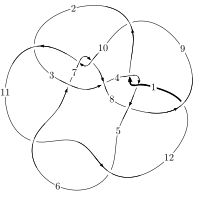
\includegraphics[width=112pt]{../../../GIT/diagram.site/Diagrams/png/2007_12a_1206.png}\\
\ \ \ A knot diagram\footnotemark}&
\allowdisplaybreaks
\textbf{Linearized knot diagam} \\
\cline{2-2}
 &
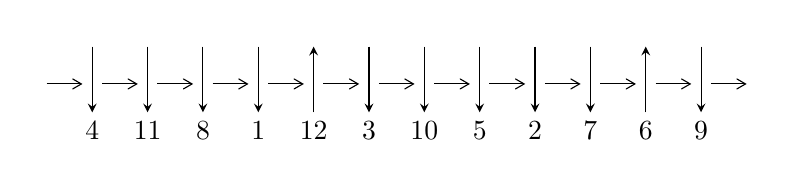
\begin{tikzpicture}[x=20pt, y=17pt]
	% nodes
	\node (C0) at (0, 0) {};
	\node (C1) at (1, 0) {};
	\node (C1U) at (1, +1) {};
	\node (C1D) at (1, -1) {4};

	\node (C2) at (2, 0) {};
	\node (C2U) at (2, +1) {};
	\node (C2D) at (2, -1) {11};

	\node (C3) at (3, 0) {};
	\node (C3U) at (3, +1) {};
	\node (C3D) at (3, -1) {8};

	\node (C4) at (4, 0) {};
	\node (C4U) at (4, +1) {};
	\node (C4D) at (4, -1) {1};

	\node (C5) at (5, 0) {};
	\node (C5U) at (5, +1) {};
	\node (C5D) at (5, -1) {12};

	\node (C6) at (6, 0) {};
	\node (C6U) at (6, +1) {};
	\node (C6D) at (6, -1) {3};

	\node (C7) at (7, 0) {};
	\node (C7U) at (7, +1) {};
	\node (C7D) at (7, -1) {10};

	\node (C8) at (8, 0) {};
	\node (C8U) at (8, +1) {};
	\node (C8D) at (8, -1) {5};

	\node (C9) at (9, 0) {};
	\node (C9U) at (9, +1) {};
	\node (C9D) at (9, -1) {2};

	\node (C10) at (10, 0) {};
	\node (C10U) at (10, +1) {};
	\node (C10D) at (10, -1) {7};

	\node (C11) at (11, 0) {};
	\node (C11U) at (11, +1) {};
	\node (C11D) at (11, -1) {6};

	\node (C12) at (12, 0) {};
	\node (C12U) at (12, +1) {};
	\node (C12D) at (12, -1) {9};
	\node (C13) at (13, 0) {};

	% arrows
	\draw[->,>={angle 60}]
	(C0) edge (C1) (C1) edge (C2) (C2) edge (C3) (C3) edge (C4) (C4) edge (C5) (C5) edge (C6) (C6) edge (C7) (C7) edge (C8) (C8) edge (C9) (C9) edge (C10) (C10) edge (C11) (C11) edge (C12) (C12) edge (C13) ;	\draw[->,>=stealth]
	(C1U) edge (C1D) (C2U) edge (C2D) (C3U) edge (C3D) (C4U) edge (C4D) (C5D) edge (C5U) (C6U) edge (C6D) (C7U) edge (C7D) (C8U) edge (C8D) (C9U) edge (C9D) (C10U) edge (C10D) (C11D) edge (C11U) (C12U) edge (C12D) ;
	\end{tikzpicture} \\
\hhline{~~} \\& 
\textbf{Solving Sequence} \\ \cline{2-2} 
 &
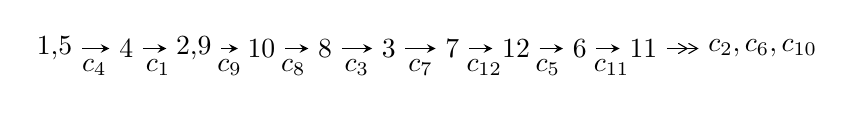
\begin{tikzpicture}[x=23pt, y=7pt]
	% node
	\node (A0) at (-1/8, 0) {1,5};
	\node (A1) at (1, 0) {4};
	\node (A2) at (33/16, 0) {2,9};
	\node (A3) at (25/8, 0) {10};
	\node (A4) at (33/8, 0) {8};
	\node (A5) at (41/8, 0) {3};
	\node (A6) at (49/8, 0) {7};
	\node (A7) at (57/8, 0) {12};
	\node (A8) at (65/8, 0) {6};
	\node (A9) at (73/8, 0) {11};
	\node (C1) at (1/2, -1) {$c_{4}$};
	\node (C2) at (3/2, -1) {$c_{1}$};
	\node (C3) at (21/8, -1) {$c_{9}$};
	\node (C4) at (29/8, -1) {$c_{8}$};
	\node (C5) at (37/8, -1) {$c_{3}$};
	\node (C6) at (45/8, -1) {$c_{7}$};
	\node (C7) at (53/8, -1) {$c_{12}$};
	\node (C8) at (61/8, -1) {$c_{5}$};
	\node (C9) at (69/8, -1) {$c_{11}$};
	\node (A10) at (11, 0) {$c_{2},c_{6},c_{10}$};

	% edge
	\draw[->,>=stealth]	
	(A0) edge (A1) (A1) edge (A2) (A2) edge (A3) (A3) edge (A4) (A4) edge (A5) (A5) edge (A6) (A6) edge (A7) (A7) edge (A8) (A8) edge (A9) ;
	\draw[->>,>={angle 60}]	
	(A9) edge (A10);
\end{tikzpicture} \\ 

\end{tabular} \\

\footnotetext{
The image of knot diagram is generated by the software ``\textbf{Draw programme}" developed by Andrew Bartholomew(\url{http://www.layer8.co.uk/maths/draw/index.htm\#Running-draw}), where we modified some parts for our purpose(\url{https://github.com/CATsTAILs/LinksPainter}).
}\phantom \\ \newline 
\centering \textbf{Ideals for irreducible components\footnotemark of $X_{\text{par}}$} 
 
\begin{align*}
I^u_{1}&=\langle 
-3 u^{18}+21 u^{17}+\cdots+4 b+12,\;3 u^{18}-15 u^{17}+\cdots+8 a+60,\;u^{19}-7 u^{18}+\cdots-36 u+8\rangle \\
I^u_{2}&=\langle 
-992688 u^{27}+12625506 u^{26}+\cdots+34453 b+67406583,\\
\phantom{I^u_{2}}&\phantom{= \langle  }67406583 u^{27}-859313682 u^{26}+\cdots+2928505 a-5202887920,\;u^{28}-14 u^{27}+\cdots-855 u+85\rangle \\
I^u_{3}&=\langle 
545822815415 u^{11} a^5-8124336604603 u^{11} a^4+\cdots-7690591677159 a+38068629937764,\\
\phantom{I^u_{3}}&\phantom{= \langle  }-3 u^{11} a^4+u^{11} a^3+\cdots+21 a+95,\\
\phantom{I^u_{3}}&\phantom{= \langle  }u^{12}+3 u^{11}+8 u^{10}+13 u^9+18 u^8+21 u^7+19 u^6+17 u^5+10 u^4+6 u^3+4 u^2+1\rangle \\
I^u_{4}&=\langle 
-15385 u^{25}-30619 u^{24}+\cdots+143017 b+1607536,\\
\phantom{I^u_{4}}&\phantom{= \langle  }-229648 u^{25}-1852569 u^{24}+\cdots+143017 a-478848,\;u^{26}+8 u^{25}+\cdots+62 u+7\rangle \\
I^u_{5}&=\langle 
- a^3 u^2+a^3 u- a^2 u^2+a^3-2 a^2 u-2 u^2 a- a^2-6 a u+2 u^2+2 b-2 a+u+2,\\
\phantom{I^u_{5}}&\phantom{= \langle  }a^3 u^2+a^4+2 a^3-2 a^2 u+3 u^2 a- a^2+a u+10 u^2+5 a+5 u+17,\;u^3+u^2+2 u+1\rangle \\
I^u_{6}&=\langle 
-9 a^5 u-20 a^5+14 a^4 u-31 a^4+73 a^3 u+38 a^3-18 a^2 u+46 a^2-82 a u+43 b-15 a-17 u-33,\\
\phantom{I^u_{6}}&\phantom{= \langle  }a^6- a^5 u-2 a^4 u-3 a^4+3 a^3 u+2 a^3+a^2 u- a^2-2 a u+a+u+1,\;u^2+u+1\rangle \\
I^u_{7}&=\langle 
- u^2+b- u-1,\;u^2+a+1,\;u^3+u^2+2 u+1\rangle \\
I^u_{8}&=\langle 
b,\;a-1,\;u^3+u^2+2 u+1\rangle \\
I^u_{9}&=\langle 
b+u,\;a,\;u^3+u^2+2 u+1\rangle \\
I^u_{10}&=\langle 
b+u,\;a-1,\;u^2- u+1\rangle \\
\\
\end{align*}
\raggedright * 10 irreducible components of $\dim_{\mathbb{C}}=0$, with total 180 representations.\\
\footnotetext{All coefficients of polynomials are rational numbers. But the coefficients are sometimes approximated in decimal forms when there is not enough margin.}
\newpage
\renewcommand{\arraystretch}{1}
\centering \section*{I. $I^u_{1}= \langle -3 u^{18}+21 u^{17}+\cdots+4 b+12,\;3 u^{18}-15 u^{17}+\cdots+8 a+60,\;u^{19}-7 u^{18}+\cdots-36 u+8 \rangle$}
\flushleft \textbf{(i) Arc colorings}\\
\begin{tabular}{m{7pt} m{180pt} m{7pt} m{180pt} }
\flushright $a_{1}=$&$\begin{pmatrix}0\\u\end{pmatrix}$ \\
\flushright $a_{5}=$&$\begin{pmatrix}1\\0\end{pmatrix}$ \\
\flushright $a_{4}=$&$\begin{pmatrix}1\\- u^2\end{pmatrix}$ \\
\flushright $a_{2}=$&$\begin{pmatrix}- u\\u^3+u\end{pmatrix}$ \\
\flushright $a_{9}=$&$\begin{pmatrix}-0.375000 u^{18}+1.87500 u^{17}+\cdots+29.7500 u-7.50000\\\frac{3}{4} u^{18}-\frac{21}{4} u^{17}+\cdots+21 u-3\end{pmatrix}$ \\
\flushright $a_{10}=$&$\begin{pmatrix}-\frac{3}{8} u^{18}+\frac{7}{8} u^{17}+\cdots+\frac{239}{4} u-\frac{27}{2}\\-\frac{1}{4} u^{18}-\frac{1}{4} u^{17}+\cdots+27 u-5\end{pmatrix}$ \\
\flushright $a_{8}=$&$\begin{pmatrix}\frac{3}{8} u^{18}-\frac{27}{8} u^{17}+\cdots+\frac{203}{4} u-\frac{21}{2}\\\frac{3}{4} u^{18}-\frac{21}{4} u^{17}+\cdots+21 u-3\end{pmatrix}$ \\
\flushright $a_{3}=$&$\begin{pmatrix}\frac{5}{8} u^{18}-\frac{37}{8} u^{17}+\cdots+\frac{83}{4} u-3\\\frac{3}{4} u^{18}-\frac{19}{4} u^{17}+\cdots+\frac{15}{2} u-1\end{pmatrix}$ \\
\flushright $a_{7}=$&$\begin{pmatrix}-1.37500 u^{18}+9.87500 u^{17}+\cdots+23.7500 u-7.50000\\-\frac{5}{4} u^{18}+\frac{31}{4} u^{17}+\cdots+7 u-1\end{pmatrix}$ \\
\flushright $a_{12}=$&$\begin{pmatrix}-\frac{7}{8} u^{18}+\frac{47}{8} u^{17}+\cdots-\frac{57}{4} u+2\\\frac{1}{4} u^{18}-\frac{9}{4} u^{17}+\cdots+\frac{61}{2} u-7\end{pmatrix}$ \\
\flushright $a_{6}=$&$\begin{pmatrix}\frac{7}{8} u^{18}-\frac{37}{8} u^{17}+\cdots-\frac{25}{2} u+3\\- u^{18}+\frac{15}{2} u^{17}+\cdots-\frac{71}{2} u+9\end{pmatrix}$ \\
\flushright $a_{11}=$&$\begin{pmatrix}\frac{1}{8} u^{18}-\frac{17}{8} u^{17}+\cdots-\frac{11}{4} u+\frac{5}{2}\\\frac{5}{4} u^{18}-\frac{35}{4} u^{17}+\cdots+19 u-5\end{pmatrix}$\\&\end{tabular}
\flushleft \textbf{(ii) Obstruction class $= -1$}\\~\\
\flushleft \textbf{(iii) Cusp Shapes $= u^{18}-7 u^{17}+28 u^{16}-77 u^{15}+159 u^{14}-256 u^{13}+322 u^{12}-304 u^{11}+174 u^{10}+38 u^9-247 u^8+357 u^7-324 u^6+183 u^5-32 u^4-69 u^3+81 u^2-50 u+10$}\\~\\
\newpage\renewcommand{\arraystretch}{1}
\flushleft \textbf{(iv) u-Polynomials at the component}\newline \\
\begin{tabular}{m{50pt}|m{274pt}}
Crossings & \hspace{64pt}u-Polynomials at each crossing \\
\hline $$\begin{aligned}c_{1},c_{4},c_{7}\\c_{10}\end{aligned}$$&$\begin{aligned}
&u^{19}-7 u^{18}+\cdots-36 u+8
\end{aligned}$\\
\hline $$\begin{aligned}c_{2},c_{6},c_{8}\\c_{12}\end{aligned}$$&$\begin{aligned}
&u^{19}+2 u^{17}+\cdots+5 u+1
\end{aligned}$\\
\hline $$\begin{aligned}c_{3},c_{9}\end{aligned}$$&$\begin{aligned}
&u^{19}-5 u^{18}+\cdots+22 u+12
\end{aligned}$\\
\hline $$\begin{aligned}c_{5},c_{11}\end{aligned}$$&$\begin{aligned}
&u^{19}-11 u^{18}+\cdots-224 u+32
\end{aligned}$\\
\hline
\end{tabular}\\~\\
\newpage\renewcommand{\arraystretch}{1}
\flushleft \textbf{(v) Riley Polynomials at the component}\newline \\
\begin{tabular}{m{50pt}|m{274pt}}
Crossings & \hspace{64pt}Riley Polynomials at each crossing \\
\hline $$\begin{aligned}c_{1},c_{4},c_{7}\\c_{10}\end{aligned}$$&$\begin{aligned}
&y^{19}+11 y^{18}+\cdots-304 y-64
\end{aligned}$\\
\hline $$\begin{aligned}c_{2},c_{6},c_{8}\\c_{12}\end{aligned}$$&$\begin{aligned}
&y^{19}+4 y^{18}+\cdots+5 y-1
\end{aligned}$\\
\hline $$\begin{aligned}c_{3},c_{9}\end{aligned}$$&$\begin{aligned}
&y^{19}-15 y^{18}+\cdots-164 y-144
\end{aligned}$\\
\hline $$\begin{aligned}c_{5},c_{11}\end{aligned}$$&$\begin{aligned}
&y^{19}+9 y^{18}+\cdots+512 y-1024
\end{aligned}$\\
\hline
\end{tabular}\\~\\
\newpage\flushleft \textbf{(vi) Complex Volumes and Cusp Shapes}
$$\begin{array}{c|c|c}  
\text{Solutions to }I^u_{1}& \I (\text{vol} + \sqrt{-1}CS) & \text{Cusp shape}\\
 \hline 
\begin{aligned}
u &= -0.089256 + 1.007980 I \\
a &= \phantom{-}1.05363 - 1.09151 I \\
b &= -1.00618 - 1.15946 I\end{aligned}
 & \phantom{-}0.28070 - 2.38140 I & -5.46513 + 2.98597 I \\ \hline\begin{aligned}
u &= -0.089256 - 1.007980 I \\
a &= \phantom{-}1.05363 + 1.09151 I \\
b &= -1.00618 + 1.15946 I\end{aligned}
 & \phantom{-}0.28070 + 2.38140 I & -5.46513 - 2.98597 I \\ \hline\begin{aligned}
u &= -0.129693 + 1.056200 I \\
a &= -0.901489 + 0.653587 I \\
b &= \phantom{-}0.573401 + 1.036920 I\end{aligned}
 & \phantom{-}4.83655 + 0.75731 I & \phantom{-}0.29531 + 1.48803 I \\ \hline\begin{aligned}
u &= -0.129693 - 1.056200 I \\
a &= -0.901489 - 0.653587 I \\
b &= \phantom{-}0.573401 - 1.036920 I\end{aligned}
 & \phantom{-}4.83655 - 0.75731 I & \phantom{-}0.29531 - 1.48803 I \\ \hline\begin{aligned}
u &= \phantom{-}1.070160 + 0.136306 I \\
a &= \phantom{-}0.880972 - 0.767951 I \\
b &= -1.047450 + 0.701745 I\end{aligned}
 & -8.89959 + 8.35587 I & -14.4938 - 6.1627 I \\ \hline\begin{aligned}
u &= \phantom{-}1.070160 - 0.136306 I \\
a &= \phantom{-}0.880972 + 0.767951 I \\
b &= -1.047450 - 0.701745 I\end{aligned}
 & -8.89959 - 8.35587 I & -14.4938 + 6.1627 I \\ \hline\begin{aligned}
u &= -0.283957 + 1.128460 I \\
a &= \phantom{-}0.468063 - 0.377219 I \\
b &= -0.292767 - 0.635305 I\end{aligned}
 & \phantom{-}2.62810 + 3.46250 I & -5.41765 - 4.29370 I \\ \hline\begin{aligned}
u &= -0.283957 - 1.128460 I \\
a &= \phantom{-}0.468063 + 0.377219 I \\
b &= -0.292767 + 0.635305 I\end{aligned}
 & \phantom{-}2.62810 - 3.46250 I & -5.41765 + 4.29370 I \\ \hline\begin{aligned}
u &= \phantom{-}1.041110 + 0.527820 I \\
a &= -0.102160 + 0.634385 I \\
b &= \phantom{-}0.441200 - 0.606542 I\end{aligned}
 & -1.27781 + 2.04691 I & -4.21735 - 12.06061 I \\ \hline\begin{aligned}
u &= \phantom{-}1.041110 - 0.527820 I \\
a &= -0.102160 - 0.634385 I \\
b &= \phantom{-}0.441200 + 0.606542 I\end{aligned}
 & -1.27781 - 2.04691 I & -4.21735 + 12.06061 I\\
 \hline 
 \end{array}$$\newpage$$\begin{array}{c|c|c}  
\text{Solutions to }I^u_{1}& \I (\text{vol} + \sqrt{-1}CS) & \text{Cusp shape}\\
 \hline 
\begin{aligned}
u &= -0.726236\phantom{ +0.000000I} \\
a &= \phantom{-}0.400633\phantom{ +0.000000I} \\
b &= \phantom{-}0.290954\phantom{ +0.000000I}\end{aligned}
 & -1.16657\phantom{ +0.000000I} & -7.54420\phantom{ +0.000000I} \\ \hline\begin{aligned}
u &= \phantom{-}0.311802 + 0.537677 I \\
a &= \phantom{-}0.371981 + 1.120770 I \\
b &= \phantom{-}0.486627 - 0.549464 I\end{aligned}
 & -0.73404 + 1.68177 I & -4.58767 - 4.23908 I \\ \hline\begin{aligned}
u &= \phantom{-}0.311802 - 0.537677 I \\
a &= \phantom{-}0.371981 - 1.120770 I \\
b &= \phantom{-}0.486627 + 0.549464 I\end{aligned}
 & -0.73404 - 1.68177 I & -4.58767 + 4.23908 I \\ \hline\begin{aligned}
u &= \phantom{-}0.56617 + 1.36797 I \\
a &= -1.054680 + 0.464599 I \\
b &= \phantom{-}1.23269 + 1.17973 I\end{aligned}
 & -1.0494 - 20.1774 I & -7.61137 + 10.06897 I \\ \hline\begin{aligned}
u &= \phantom{-}0.56617 - 1.36797 I \\
a &= -1.054680 - 0.464599 I \\
b &= \phantom{-}1.23269 - 1.17973 I\end{aligned}
 & -1.0494 + 20.1774 I & -7.61137 - 10.06897 I \\ \hline\begin{aligned}
u &= \phantom{-}0.61070 + 1.36309 I \\
a &= \phantom{-}0.904319 - 0.205921 I \\
b &= -0.832955 - 1.106920 I\end{aligned}
 & \phantom{-}5.3054 - 14.5379 I & -4.33039 + 10.14035 I \\ \hline\begin{aligned}
u &= \phantom{-}0.61070 - 1.36309 I \\
a &= \phantom{-}0.904319 + 0.205921 I \\
b &= -0.832955 + 1.106920 I\end{aligned}
 & \phantom{-}5.3054 + 14.5379 I & -4.33039 - 10.14035 I \\ \hline\begin{aligned}
u &= \phantom{-}0.76609 + 1.32486 I \\
a &= -0.570950 - 0.103738 I \\
b &= \phantom{-}0.299958 + 0.835901 I\end{aligned}
 & \phantom{-}4.42824 - 6.79161 I & \phantom{-}0.60019 + 10.60796 I \\ \hline\begin{aligned}
u &= \phantom{-}0.76609 - 1.32486 I \\
a &= -0.570950 + 0.103738 I \\
b &= \phantom{-}0.299958 - 0.835901 I\end{aligned}
 & \phantom{-}4.42824 + 6.79161 I & \phantom{-}0.60019 - 10.60796 I\\
 \hline 
 \end{array}$$\newpage\newpage\renewcommand{\arraystretch}{1}
\centering \section*{II. $I^u_{2}= \langle -9.93\times10^{5} u^{27}+1.26\times10^{7} u^{26}+\cdots+3.45\times10^{4} b+6.74\times10^{7},\;6.74\times10^{7} u^{27}-8.59\times10^{8} u^{26}+\cdots+2.93\times10^{6} a-5.20\times10^{9},\;u^{28}-14 u^{27}+\cdots-855 u+85 \rangle$}
\flushleft \textbf{(i) Arc colorings}\\
\begin{tabular}{m{7pt} m{180pt} m{7pt} m{180pt} }
\flushright $a_{1}=$&$\begin{pmatrix}0\\u\end{pmatrix}$ \\
\flushright $a_{5}=$&$\begin{pmatrix}1\\0\end{pmatrix}$ \\
\flushright $a_{4}=$&$\begin{pmatrix}1\\- u^2\end{pmatrix}$ \\
\flushright $a_{2}=$&$\begin{pmatrix}- u\\u^3+u\end{pmatrix}$ \\
\flushright $a_{9}=$&$\begin{pmatrix}-23.0174 u^{27}+293.431 u^{26}+\cdots-16206.9 u+1776.64\\28.8128 u^{27}-366.456 u^{26}+\cdots+17903.2 u-1956.48\end{pmatrix}$ \\
\flushright $a_{10}=$&$\begin{pmatrix}15.6733 u^{27}-202.020 u^{26}+\cdots+10608.3 u-1152.25\\-66.8738 u^{27}+859.315 u^{26}+\cdots-45141.3 u+4901.10\end{pmatrix}$ \\
\flushright $a_{8}=$&$\begin{pmatrix}5.79541 u^{27}-73.0251 u^{26}+\cdots+1696.29 u-179.843\\28.8128 u^{27}-366.456 u^{26}+\cdots+17903.2 u-1956.48\end{pmatrix}$ \\
\flushright $a_{3}=$&$\begin{pmatrix}-10.2277 u^{27}+130.845 u^{26}+\cdots-6911.51 u+756.352\\-76.4924 u^{27}+982.058 u^{26}+\cdots-51779.1 u+5632.50\end{pmatrix}$ \\
\flushright $a_{7}=$&$\begin{pmatrix}45.0001 u^{27}-576.476 u^{26}+\cdots+28129.0 u-3053.06\\-140.536 u^{27}+1807.65 u^{26}+\cdots-95332.1 u+10352.0\end{pmatrix}$ \\
\flushright $a_{12}=$&$\begin{pmatrix}54.3698 u^{27}-696.998 u^{26}+\cdots+37058.1 u-4043.28\\-64.1800 u^{27}+822.445 u^{26}+\cdots-42441.9 u+4621.44\end{pmatrix}$ \\
\flushright $a_{6}=$&$\begin{pmatrix}14.5690 u^{27}-185.347 u^{26}+\cdots+7527.26 u-813.539\\57.4557 u^{27}-734.448 u^{26}+\cdots+38610.4 u-4216.93\end{pmatrix}$ \\
\flushright $a_{11}=$&$\begin{pmatrix}-36.9975 u^{27}+469.587 u^{26}+\cdots-23688.5 u+2597.06\\54.5215 u^{27}-700.386 u^{26}+\cdots+34381.6 u-3716.35\end{pmatrix}$\\&\end{tabular}
\flushleft \textbf{(ii) Obstruction class $= -1$}\\~\\
\flushleft \textbf{(iii) Cusp Shapes $= \frac{12799129}{34453} u^{27}-\frac{164577489}{34453} u^{26}+\cdots+\frac{8305113305}{34453} u-\frac{900475230}{34453}$}\\~\\
\newpage\renewcommand{\arraystretch}{1}
\flushleft \textbf{(iv) u-Polynomials at the component}\newline \\
\begin{tabular}{m{50pt}|m{274pt}}
Crossings & \hspace{64pt}u-Polynomials at each crossing \\
\hline $$\begin{aligned}c_{1},c_{4},c_{7}\\c_{10}\end{aligned}$$&$\begin{aligned}
&u^{28}-14 u^{27}+\cdots-855 u+85
\end{aligned}$\\
\hline $$\begin{aligned}c_{2},c_{6},c_{8}\\c_{12}\end{aligned}$$&$\begin{aligned}
&u^{28}+4 u^{27}+\cdots-2 u+1
\end{aligned}$\\
\hline $$\begin{aligned}c_{3},c_{9}\end{aligned}$$&$\begin{aligned}
&(u^{14}+2 u^{13}+\cdots- u+1)^{2}
\end{aligned}$\\
\hline $$\begin{aligned}c_{5},c_{11}\end{aligned}$$&$\begin{aligned}
&(u^{14}-9 u^{13}+\cdots-416 u+64)^{2}
\end{aligned}$\\
\hline
\end{tabular}\\~\\
\newpage\renewcommand{\arraystretch}{1}
\flushleft \textbf{(v) Riley Polynomials at the component}\newline \\
\begin{tabular}{m{50pt}|m{274pt}}
Crossings & \hspace{64pt}Riley Polynomials at each crossing \\
\hline $$\begin{aligned}c_{1},c_{4},c_{7}\\c_{10}\end{aligned}$$&$\begin{aligned}
&y^{28}+22 y^{27}+\cdots+79025 y+7225
\end{aligned}$\\
\hline $$\begin{aligned}c_{2},c_{6},c_{8}\\c_{12}\end{aligned}$$&$\begin{aligned}
&y^{28}+4 y^{27}+\cdots-10 y+1
\end{aligned}$\\
\hline $$\begin{aligned}c_{3},c_{9}\end{aligned}$$&$\begin{aligned}
&(y^{14}+4 y^{12}+\cdots-3 y+1)^{2}
\end{aligned}$\\
\hline $$\begin{aligned}c_{5},c_{11}\end{aligned}$$&$\begin{aligned}
&(y^{14}+15 y^{13}+\cdots-5120 y+4096)^{2}
\end{aligned}$\\
\hline
\end{tabular}\\~\\
\newpage\flushleft \textbf{(vi) Complex Volumes and Cusp Shapes}
$$\begin{array}{c|c|c}  
\text{Solutions to }I^u_{2}& \I (\text{vol} + \sqrt{-1}CS) & \text{Cusp shape}\\
 \hline 
\begin{aligned}
u &= \phantom{-}0.220870 + 0.964019 I \\
a &= \phantom{-}0.976311 - 0.269060 I \\
b &= -0.475016 - 0.881755 I\end{aligned}
 & \phantom{-}3.33157 - 0.04587 I & \phantom{-0.000000 } 0 \\ \hline\begin{aligned}
u &= \phantom{-}0.220870 - 0.964019 I \\
a &= \phantom{-}0.976311 + 0.269060 I \\
b &= -0.475016 + 0.881755 I\end{aligned}
 & \phantom{-}3.33157 + 0.04587 I & \phantom{-0.000000 } 0 \\ \hline\begin{aligned}
u &= \phantom{-}0.122015 + 0.951919 I \\
a &= -1.22987 + 0.91180 I \\
b &= \phantom{-}1.01802 + 1.05948 I\end{aligned}
 & -0.07368 - 3.51148 I & -8.00000 + 0. I\phantom{ +0.000000I} \\ \hline\begin{aligned}
u &= \phantom{-}0.122015 - 0.951919 I \\
a &= -1.22987 - 0.91180 I \\
b &= \phantom{-}1.01802 - 1.05948 I\end{aligned}
 & -0.07368 + 3.51148 I & -8.00000 + 0. I\phantom{ +0.000000I} \\ \hline\begin{aligned}
u &= -0.244537 + 0.840894 I \\
a &= -0.869115 - 0.048582 I \\
b &= -0.253383 + 0.718954 I\end{aligned}
 & -0.07368 + 3.51148 I & -8.00000 - 3.11087 I \\ \hline\begin{aligned}
u &= -0.244537 - 0.840894 I \\
a &= -0.869115 + 0.048582 I \\
b &= -0.253383 - 0.718954 I\end{aligned}
 & -0.07368 - 3.51148 I & -8.00000 + 3.11087 I \\ \hline\begin{aligned}
u &= \phantom{-}1.160470 + 0.000299 I \\
a &= -0.944468 - 0.613736 I \\
b &= \phantom{-}1.095850 + 0.712507 I\end{aligned}
 & -5.3108 - 14.1347 I & \phantom{-0.000000 } 0 \\ \hline\begin{aligned}
u &= \phantom{-}1.160470 - 0.000299 I \\
a &= -0.944468 + 0.613736 I \\
b &= \phantom{-}1.095850 - 0.712507 I\end{aligned}
 & -5.3108 + 14.1347 I & \phantom{-0.000000 } 0 \\ \hline\begin{aligned}
u &= \phantom{-}0.725406 + 0.404321 I \\
a &= -0.59123 + 1.38586 I \\
b &= \phantom{-}0.989219 - 0.766265 I\end{aligned}
 & -3.19044 + 2.69182 I & -19.3369 - 28.0122 I \\ \hline\begin{aligned}
u &= \phantom{-}0.725406 - 0.404321 I \\
a &= -0.59123 - 1.38586 I \\
b &= \phantom{-}0.989219 + 0.766265 I\end{aligned}
 & -3.19044 - 2.69182 I & -19.3369 + 28.0122 I\\
 \hline 
 \end{array}$$\newpage$$\begin{array}{c|c|c}  
\text{Solutions to }I^u_{2}& \I (\text{vol} + \sqrt{-1}CS) & \text{Cusp shape}\\
 \hline 
\begin{aligned}
u &= \phantom{-}0.493746 + 1.144530 I \\
a &= -1.266750 + 0.472811 I \\
b &= \phantom{-}1.16660 + 1.21638 I\end{aligned}
 & -0.82954 - 7.36918 I & \phantom{-0.000000 } 0 \\ \hline\begin{aligned}
u &= \phantom{-}0.493746 - 1.144530 I \\
a &= -1.266750 - 0.472811 I \\
b &= \phantom{-}1.16660 - 1.21638 I\end{aligned}
 & -0.82954 + 7.36918 I & \phantom{-0.000000 } 0 \\ \hline\begin{aligned}
u &= \phantom{-}0.288974 + 1.259790 I \\
a &= \phantom{-}0.981923 - 0.455892 I \\
b &= -0.858078 - 1.105270 I\end{aligned}
 & \phantom{-}8.09763 - 2.64325 I & \phantom{-0.000000 } 0 \\ \hline\begin{aligned}
u &= \phantom{-}0.288974 - 1.259790 I \\
a &= \phantom{-}0.981923 + 0.455892 I \\
b &= -0.858078 + 1.105270 I\end{aligned}
 & \phantom{-}8.09763 + 2.64325 I & \phantom{-0.000000 } 0 \\ \hline\begin{aligned}
u &= \phantom{-}0.601682 + 1.216810 I \\
a &= -1.019270 + 0.137827 I \\
b &= \phantom{-}0.780986 + 1.157340 I\end{aligned}
 & \phantom{-}1.26514 - 7.93875 I & \phantom{-0.000000 } 0 \\ \hline\begin{aligned}
u &= \phantom{-}0.601682 - 1.216810 I \\
a &= -1.019270 - 0.137827 I \\
b &= \phantom{-}0.780986 - 1.157340 I\end{aligned}
 & \phantom{-}1.26514 + 7.93875 I & \phantom{-0.000000 } 0 \\ \hline\begin{aligned}
u &= \phantom{-}1.366350 + 0.089976 I \\
a &= \phantom{-}0.354535 - 0.376999 I \\
b &= -0.518338 + 0.483212 I\end{aligned}
 & \phantom{-}1.26514 + 7.93875 I & \phantom{-0.000000 } 0 \\ \hline\begin{aligned}
u &= \phantom{-}1.366350 - 0.089976 I \\
a &= \phantom{-}0.354535 + 0.376999 I \\
b &= -0.518338 - 0.483212 I\end{aligned}
 & \phantom{-}1.26514 - 7.93875 I & \phantom{-0.000000 } 0 \\ \hline\begin{aligned}
u &= \phantom{-}0.567715 + 1.286990 I \\
a &= \phantom{-}1.111150 - 0.453605 I \\
b &= -1.21460 - 1.17252 I\end{aligned}
 & -5.3108 - 14.1347 I & \phantom{-0.000000 } 0 \\ \hline\begin{aligned}
u &= \phantom{-}0.567715 - 1.286990 I \\
a &= \phantom{-}1.111150 + 0.453605 I \\
b &= -1.21460 + 1.17252 I\end{aligned}
 & -5.3108 + 14.1347 I & \phantom{-0.000000 } 0\\
 \hline 
 \end{array}$$\newpage$$\begin{array}{c|c|c}  
\text{Solutions to }I^u_{2}& \I (\text{vol} + \sqrt{-1}CS) & \text{Cusp shape}\\
 \hline 
\begin{aligned}
u &= \phantom{-}0.250099 + 0.518873 I \\
a &= \phantom{-}1.58195 + 0.00658 I \\
b &= -0.392229 - 0.822475 I\end{aligned}
 & \phantom{-}3.33157 + 0.04587 I & -1.17760 + 1.07149 I \\ \hline\begin{aligned}
u &= \phantom{-}0.250099 - 0.518873 I \\
a &= \phantom{-}1.58195 - 0.00658 I \\
b &= -0.392229 + 0.822475 I\end{aligned}
 & \phantom{-}3.33157 - 0.04587 I & -1.17760 - 1.07149 I \\ \hline\begin{aligned}
u &= \phantom{-}0.24300 + 1.41025 I \\
a &= -0.643805 + 0.208891 I \\
b &= \phantom{-}0.451032 + 0.857168 I\end{aligned}
 & \phantom{-}8.09763 + 2.64325 I & \phantom{-0.000000 } 0 \\ \hline\begin{aligned}
u &= \phantom{-}0.24300 - 1.41025 I \\
a &= -0.643805 - 0.208891 I \\
b &= \phantom{-}0.451032 - 0.857168 I\end{aligned}
 & \phantom{-}8.09763 - 2.64325 I & \phantom{-0.000000 } 0 \\ \hline\begin{aligned}
u &= \phantom{-}0.82492 + 1.56847 I \\
a &= -0.060677 + 0.273569 I \\
b &= \phantom{-}0.479139 - 0.130503 I\end{aligned}
 & -0.82954 + 7.36918 I & \phantom{-0.000000 } 0 \\ \hline\begin{aligned}
u &= \phantom{-}0.82492 - 1.56847 I \\
a &= -0.060677 - 0.273569 I \\
b &= \phantom{-}0.479139 + 0.130503 I\end{aligned}
 & -0.82954 - 7.36918 I & \phantom{-0.000000 } 0 \\ \hline\begin{aligned}
u &= \phantom{-}0.37929 + 1.83155 I \\
a &= -0.057146 - 0.158811 I \\
b &= -0.269196 + 0.164900 I\end{aligned}
 & -3.19044 + 2.69182 I & \phantom{-0.000000 } 0 \\ \hline\begin{aligned}
u &= \phantom{-}0.37929 - 1.83155 I \\
a &= -0.057146 + 0.158811 I \\
b &= -0.269196 - 0.164900 I\end{aligned}
 & -3.19044 - 2.69182 I & \phantom{-0.000000 } 0\\
 \hline 
 \end{array}$$\newpage\newpage\renewcommand{\arraystretch}{1}
\centering \section*{III. $I^u_{3}= \langle 5.46\times10^{11} a^{5} u^{11}-8.12\times10^{12} a^{4} u^{11}+\cdots-7.69\times10^{12} a+3.81\times10^{13},\;-3 u^{11} a^4+u^{11} a^3+\cdots+21 a+95,\;u^{12}+3 u^{11}+\cdots+4 u^2+1 \rangle$}
\flushleft \textbf{(i) Arc colorings}\\
\begin{tabular}{m{7pt} m{180pt} m{7pt} m{180pt} }
\flushright $a_{1}=$&$\begin{pmatrix}0\\u\end{pmatrix}$ \\
\flushright $a_{5}=$&$\begin{pmatrix}1\\0\end{pmatrix}$ \\
\flushright $a_{4}=$&$\begin{pmatrix}1\\- u^2\end{pmatrix}$ \\
\flushright $a_{2}=$&$\begin{pmatrix}- u\\u^3+u\end{pmatrix}$ \\
\flushright $a_{9}=$&$\begin{pmatrix}a\\-0.0661105 a^{5} u^{11}+0.984027 a^{4} u^{11}+\cdots+0.931491 a-4.61091\end{pmatrix}$ \\
\flushright $a_{10}=$&$\begin{pmatrix}-0.141190 a^{5} u^{11}+0.271994 a^{4} u^{11}+\cdots+1.47180 a-3.20730\\-0.292464 a^{5} u^{11}+0.0577256 a^{4} u^{11}+\cdots+0.826930 a-2.94212\end{pmatrix}$ \\
\flushright $a_{8}=$&$\begin{pmatrix}-0.0661105 a^{5} u^{11}+0.984027 a^{4} u^{11}+\cdots+1.93149 a-4.61091\\-0.0661105 a^{5} u^{11}+0.984027 a^{4} u^{11}+\cdots+0.931491 a-4.61091\end{pmatrix}$ \\
\flushright $a_{3}=$&$\begin{pmatrix}-1.03112 a^{5} u^{11}-0.0958048 a^{4} u^{11}+\cdots-3.35664 a-3.06813\\-0.807877 a^{5} u^{11}+0.0734221 a^{4} u^{11}+\cdots-2.59366 a-0.289458\end{pmatrix}$ \\
\flushright $a_{7}=$&$\begin{pmatrix}-0.300034 a^{5} u^{11}+0.348634 a^{4} u^{11}+\cdots+1.91449 a-1.62119\\-0.528393 a^{5} u^{11}+0.238256 a^{4} u^{11}+\cdots-0.0490275 a+0.579304\end{pmatrix}$ \\
\flushright $a_{12}=$&$\begin{pmatrix}a^2 u\\-0.619812 a^{5} u^{11}-0.0748662 a^{4} u^{11}+\cdots-0.523197 a+1.74280\end{pmatrix}$ \\
\flushright $a_{6}=$&$\begin{pmatrix}-0.418102 a^{5} u^{11}-0.227140 a^{4} u^{11}+\cdots-1.99363 a-0.387884\\-0.0626009 a^{5} u^{11}+0.0471036 a^{4} u^{11}+\cdots-0.374182 a+2.20004\end{pmatrix}$ \\
\flushright $a_{11}=$&$\begin{pmatrix}0.348882 a^{5} u^{11}-0.0682222 a^{4} u^{11}+\cdots-0.105524 a-2.43122\\0.557211 a^{5} u^{11}+0.121970 a^{4} u^{11}+\cdots+0.149015 a-0.542756\end{pmatrix}$\\&\end{tabular}
\flushleft \textbf{(ii) Obstruction class $= -1$}\\~\\
\flushleft \textbf{(iii) Cusp Shapes $= -\frac{18401813591608}{8256215143297} u^{11} a^5-\frac{4028033611868}{8256215143297} u^{11} a^4+\cdots-\frac{4921195373544}{8256215143297} a-\frac{130687438596918}{8256215143297}$}\\~\\
\newpage\renewcommand{\arraystretch}{1}
\flushleft \textbf{(iv) u-Polynomials at the component}\newline \\
\begin{tabular}{m{50pt}|m{274pt}}
Crossings & \hspace{64pt}u-Polynomials at each crossing \\
\hline $$\begin{aligned}c_{1},c_{4},c_{7}\\c_{10}\end{aligned}$$&$\begin{aligned}
&(u^{12}+3 u^{11}+\cdots+4 u^2+1)^{6}
\end{aligned}$\\
\hline $$\begin{aligned}c_{2},c_{6},c_{8}\\c_{12}\end{aligned}$$&$\begin{aligned}
&u^{72}+3 u^{71}+\cdots+354 u+59
\end{aligned}$\\
\hline $$\begin{aligned}c_{3},c_{9}\end{aligned}$$&$\begin{aligned}
&(u^{36}-11 u^{34}+\cdots+1120 u+320)^{2}
\end{aligned}$\\
\hline $$\begin{aligned}c_{5},c_{11}\end{aligned}$$&$\begin{aligned}
&(u^3+u^2+2 u+1)^{24}
\end{aligned}$\\
\hline
\end{tabular}\\~\\
\newpage\renewcommand{\arraystretch}{1}
\flushleft \textbf{(v) Riley Polynomials at the component}\newline \\
\begin{tabular}{m{50pt}|m{274pt}}
Crossings & \hspace{64pt}Riley Polynomials at each crossing \\
\hline $$\begin{aligned}c_{1},c_{4},c_{7}\\c_{10}\end{aligned}$$&$\begin{aligned}
&(y^{12}+7 y^{11}+\cdots+8 y+1)^{6}
\end{aligned}$\\
\hline $$\begin{aligned}c_{2},c_{6},c_{8}\\c_{12}\end{aligned}$$&$\begin{aligned}
&y^{72}-23 y^{71}+\cdots-406510 y+3481
\end{aligned}$\\
\hline $$\begin{aligned}c_{3},c_{9}\end{aligned}$$&$\begin{aligned}
&(y^{36}-22 y^{35}+\cdots-97280 y+102400)^{2}
\end{aligned}$\\
\hline $$\begin{aligned}c_{5},c_{11}\end{aligned}$$&$\begin{aligned}
&(y^3+3 y^2+2 y-1)^{24}
\end{aligned}$\\
\hline
\end{tabular}\\~\\
\newpage\flushleft \textbf{(vi) Complex Volumes and Cusp Shapes}
$$\begin{array}{c|c|c}  
\text{Solutions to }I^u_{3}& \I (\text{vol} + \sqrt{-1}CS) & \text{Cusp shape}\\
 \hline 
\begin{aligned}
u &= \phantom{-}0.234552 + 1.002020 I \\
a &= -0.720810 + 1.054620 I \\
b &= \phantom{-}0.95349 + 1.51437 I\end{aligned}
 & -0.94621 - 4.13739 I & -9.48147 + 7.59495 I \\ \hline\begin{aligned}
u &= \phantom{-}0.234552 + 1.002020 I \\
a &= \phantom{-}0.688527 - 0.072860 I \\
b &= -1.69950 + 0.60321 I\end{aligned}
 & \phantom{-}3.19138 - 6.96551 I & -2.95220 + 10.57440 I \\ \hline\begin{aligned}
u &= \phantom{-}0.234552 + 1.002020 I \\
a &= -1.64398 + 0.56675 I \\
b &= \phantom{-}1.225820 + 0.474901 I\end{aligned}
 & -0.94621 - 4.13739 I & -9.48147 + 7.59495 I \\ \hline\begin{aligned}
u &= \phantom{-}0.234552 + 1.002020 I \\
a &= -0.19432 - 1.74157 I \\
b &= -0.234503 - 0.672828 I\end{aligned}
 & \phantom{-}3.19138 - 6.96551 I & -2.95220 + 10.57440 I \\ \hline\begin{aligned}
u &= \phantom{-}0.234552 + 1.002020 I \\
a &= -0.064271 + 0.176004 I \\
b &= \phantom{-}2.12527 - 1.85054 I\end{aligned}
 & -0.94621 - 9.79363 I & -9.4815 + 13.5538 I \\ \hline\begin{aligned}
u &= \phantom{-}0.234552 + 1.002020 I \\
a &= \phantom{-}1.28018 + 2.42066 I \\
b &= \phantom{-}0.191434 + 0.023119 I\end{aligned}
 & -0.94621 - 9.79363 I & -9.4815 + 13.5538 I \\ \hline\begin{aligned}
u &= \phantom{-}0.234552 - 1.002020 I \\
a &= -0.720810 - 1.054620 I \\
b &= \phantom{-}0.95349 - 1.51437 I\end{aligned}
 & -0.94621 + 4.13739 I & -9.48147 - 7.59495 I \\ \hline\begin{aligned}
u &= \phantom{-}0.234552 - 1.002020 I \\
a &= \phantom{-}0.688527 + 0.072860 I \\
b &= -1.69950 - 0.60321 I\end{aligned}
 & \phantom{-}3.19138 + 6.96551 I & -2.95220 - 10.57440 I \\ \hline\begin{aligned}
u &= \phantom{-}0.234552 - 1.002020 I \\
a &= -1.64398 - 0.56675 I \\
b &= \phantom{-}1.225820 - 0.474901 I\end{aligned}
 & -0.94621 + 4.13739 I & -9.48147 - 7.59495 I \\ \hline\begin{aligned}
u &= \phantom{-}0.234552 - 1.002020 I \\
a &= -0.19432 + 1.74157 I \\
b &= -0.234503 + 0.672828 I\end{aligned}
 & \phantom{-}3.19138 + 6.96551 I & -2.95220 - 10.57440 I\\
 \hline 
 \end{array}$$\newpage$$\begin{array}{c|c|c}  
\text{Solutions to }I^u_{3}& \I (\text{vol} + \sqrt{-1}CS) & \text{Cusp shape}\\
 \hline 
\begin{aligned}
u &= \phantom{-}0.234552 - 1.002020 I \\
a &= -0.064271 - 0.176004 I \\
b &= \phantom{-}2.12527 + 1.85054 I\end{aligned}
 & -0.94621 + 9.79363 I & -9.4815 - 13.5538 I \\ \hline\begin{aligned}
u &= \phantom{-}0.234552 - 1.002020 I \\
a &= \phantom{-}1.28018 - 2.42066 I \\
b &= \phantom{-}0.191434 - 0.023119 I\end{aligned}
 & -0.94621 + 9.79363 I & -9.4815 - 13.5538 I \\ \hline\begin{aligned}
u &= -1.090290 + 0.140460 I \\
a &= -1.014270 + 0.266172 I \\
b &= \phantom{-}1.17507 - 0.87900 I\end{aligned}
 & -5.72690 + 3.91075 I & -17.7913 - 8.6071 I \\ \hline\begin{aligned}
u &= -1.090290 + 0.140460 I \\
a &= \phantom{-}0.748871 + 0.516780 I \\
b &= -1.31217 - 0.63591 I\end{aligned}
 & -5.72690 - 1.74550 I & -17.7913 - 2.6482 I \\ \hline\begin{aligned}
u &= -1.090290 + 0.140460 I \\
a &= \phantom{-}0.702755 + 0.135494 I \\
b &= -0.649097 + 0.219395 I\end{aligned}
 & -1.58932 + 1.08263 I & -11.26202 - 5.62762 I \\ \hline\begin{aligned}
u &= -1.090290 + 0.140460 I \\
a &= -1.109950 - 0.726241 I \\
b &= \phantom{-}0.889075 + 0.458254 I\end{aligned}
 & -5.72690 - 1.74550 I & -17.7913 - 2.6482 I \\ \hline\begin{aligned}
u &= -1.090290 + 0.140460 I \\
a &= \phantom{-}1.162330 - 0.656465 I \\
b &= -1.068470 + 0.432670 I\end{aligned}
 & -5.72690 + 3.91075 I & -17.7913 - 8.6071 I \\ \hline\begin{aligned}
u &= -1.090290 + 0.140460 I \\
a &= -0.611124 + 0.122496 I \\
b &= \phantom{-}0.785240 + 0.049019 I\end{aligned}
 & -1.58932 + 1.08263 I & -11.26202 - 5.62762 I \\ \hline\begin{aligned}
u &= -1.090290 - 0.140460 I \\
a &= -1.014270 - 0.266172 I \\
b &= \phantom{-}1.17507 + 0.87900 I\end{aligned}
 & -5.72690 - 3.91075 I & -17.7913 + 8.6071 I \\ \hline\begin{aligned}
u &= -1.090290 - 0.140460 I \\
a &= \phantom{-}0.748871 - 0.516780 I \\
b &= -1.31217 + 0.63591 I\end{aligned}
 & -5.72690 + 1.74550 I & -17.7913 + 2.6482 I\\
 \hline 
 \end{array}$$\newpage$$\begin{array}{c|c|c}  
\text{Solutions to }I^u_{3}& \I (\text{vol} + \sqrt{-1}CS) & \text{Cusp shape}\\
 \hline 
\begin{aligned}
u &= -1.090290 - 0.140460 I \\
a &= \phantom{-}0.702755 - 0.135494 I \\
b &= -0.649097 - 0.219395 I\end{aligned}
 & -1.58932 - 1.08263 I & -11.26202 + 5.62762 I \\ \hline\begin{aligned}
u &= -1.090290 - 0.140460 I \\
a &= -1.109950 + 0.726241 I \\
b &= \phantom{-}0.889075 - 0.458254 I\end{aligned}
 & -5.72690 + 1.74550 I & -17.7913 + 2.6482 I \\ \hline\begin{aligned}
u &= -1.090290 - 0.140460 I \\
a &= \phantom{-}1.162330 + 0.656465 I \\
b &= -1.068470 - 0.432670 I\end{aligned}
 & -5.72690 - 3.91075 I & -17.7913 + 8.6071 I \\ \hline\begin{aligned}
u &= -1.090290 - 0.140460 I \\
a &= -0.611124 - 0.122496 I \\
b &= \phantom{-}0.785240 - 0.049019 I\end{aligned}
 & -1.58932 - 1.08263 I & -11.26202 + 5.62762 I \\ \hline\begin{aligned}
u &= \phantom{-}0.185688 + 0.817666 I \\
a &= -0.948598 + 0.343126 I \\
b &= \phantom{-}1.295990 - 0.229859 I\end{aligned}
 & -1.58932 - 1.08263 I & -11.26202 + 5.62762 I \\ \hline\begin{aligned}
u &= \phantom{-}0.185688 + 0.817666 I \\
a &= \phantom{-}0.344955 - 1.070660 I \\
b &= -0.62210 - 2.20652 I\end{aligned}
 & -5.72690 + 1.74550 I & -17.7913 + 2.6482 I \\ \hline\begin{aligned}
u &= \phantom{-}0.185688 + 0.817666 I \\
a &= -0.07496 + 1.56796 I \\
b &= \phantom{-}0.456706 + 0.711922 I\end{aligned}
 & -1.58932 - 1.08263 I & -11.26202 + 5.62762 I \\ \hline\begin{aligned}
u &= \phantom{-}0.185688 + 0.817666 I \\
a &= -0.067503 - 0.291607 I \\
b &= -2.28703 + 1.05977 I\end{aligned}
 & -5.72690 - 3.91075 I & -17.7913 + 8.6071 I \\ \hline\begin{aligned}
u &= \phantom{-}0.185688 + 0.817666 I \\
a &= \phantom{-}2.73052 - 0.14073 I \\
b &= -0.939496 - 0.083249 I\end{aligned}
 & -5.72690 + 1.74550 I & -17.7913 + 2.6482 I \\ \hline\begin{aligned}
u &= \phantom{-}0.185688 + 0.817666 I \\
a &= -0.62849 - 2.93974 I \\
b &= -0.225903 + 0.109343 I\end{aligned}
 & -5.72690 - 3.91075 I & -17.7913 + 8.6071 I\\
 \hline 
 \end{array}$$\newpage$$\begin{array}{c|c|c}  
\text{Solutions to }I^u_{3}& \I (\text{vol} + \sqrt{-1}CS) & \text{Cusp shape}\\
 \hline 
\begin{aligned}
u &= \phantom{-}0.185688 - 0.817666 I \\
a &= -0.948598 - 0.343126 I \\
b &= \phantom{-}1.295990 + 0.229859 I\end{aligned}
 & -1.58932 + 1.08263 I & -11.26202 - 5.62762 I \\ \hline\begin{aligned}
u &= \phantom{-}0.185688 - 0.817666 I \\
a &= \phantom{-}0.344955 + 1.070660 I \\
b &= -0.62210 + 2.20652 I\end{aligned}
 & -5.72690 - 1.74550 I & -17.7913 - 2.6482 I \\ \hline\begin{aligned}
u &= \phantom{-}0.185688 - 0.817666 I \\
a &= -0.07496 - 1.56796 I \\
b &= \phantom{-}0.456706 - 0.711922 I\end{aligned}
 & -1.58932 + 1.08263 I & -11.26202 - 5.62762 I \\ \hline\begin{aligned}
u &= \phantom{-}0.185688 - 0.817666 I \\
a &= -0.067503 + 0.291607 I \\
b &= -2.28703 - 1.05977 I\end{aligned}
 & -5.72690 + 3.91075 I & -17.7913 - 8.6071 I \\ \hline\begin{aligned}
u &= \phantom{-}0.185688 - 0.817666 I \\
a &= \phantom{-}2.73052 + 0.14073 I \\
b &= -0.939496 + 0.083249 I\end{aligned}
 & -5.72690 - 1.74550 I & -17.7913 - 2.6482 I \\ \hline\begin{aligned}
u &= \phantom{-}0.185688 - 0.817666 I \\
a &= -0.62849 + 2.93974 I \\
b &= -0.225903 - 0.109343 I\end{aligned}
 & -5.72690 + 3.91075 I & -17.7913 - 8.6071 I \\ \hline\begin{aligned}
u &= -0.529049 + 1.245360 I \\
a &= \phantom{-}0.890029 + 0.495100 I \\
b &= -1.31752 + 1.32168 I\end{aligned}
 & -2.39928 + 7.38625 I & -13.25651 - 4.74994 I \\ \hline\begin{aligned}
u &= -0.529049 + 1.245360 I \\
a &= \phantom{-}0.870453 + 0.208440 I \\
b &= -0.806758 + 0.638494 I\end{aligned}
 & \phantom{-}1.73831 + 4.55813 I & -6.72725 - 1.77049 I \\ \hline\begin{aligned}
u &= -0.529049 + 1.245360 I \\
a &= -0.667447 - 0.364270 I \\
b &= \phantom{-}0.720095 - 0.973752 I\end{aligned}
 & \phantom{-}1.73831 + 4.55813 I & -6.72725 - 1.77049 I \\ \hline\begin{aligned}
u &= -0.529049 + 1.245360 I \\
a &= \phantom{-}0.056263 + 0.623747 I \\
b &= -0.375011 + 0.044252 I\end{aligned}
 & -2.39928 + 1.73000 I & -13.25651 + 1.20895 I\\
 \hline 
 \end{array}$$\newpage$$\begin{array}{c|c|c}  
\text{Solutions to }I^u_{3}& \I (\text{vol} + \sqrt{-1}CS) & \text{Cusp shape}\\
 \hline 
\begin{aligned}
u &= -0.529049 + 1.245360 I \\
a &= -1.279760 - 0.514283 I \\
b &= \phantom{-}1.087450 - 0.846474 I\end{aligned}
 & -2.39928 + 7.38625 I & -13.25651 - 4.74994 I \\ \hline\begin{aligned}
u &= -0.529049 + 1.245360 I \\
a &= -0.138468 - 0.242303 I \\
b &= \phantom{-}0.806554 + 0.259924 I\end{aligned}
 & -2.39928 + 1.73000 I & -13.25651 + 1.20895 I \\ \hline\begin{aligned}
u &= -0.529049 - 1.245360 I \\
a &= \phantom{-}0.890029 - 0.495100 I \\
b &= -1.31752 - 1.32168 I\end{aligned}
 & -2.39928 - 7.38625 I & -13.25651 + 4.74994 I \\ \hline\begin{aligned}
u &= -0.529049 - 1.245360 I \\
a &= \phantom{-}0.870453 - 0.208440 I \\
b &= -0.806758 - 0.638494 I\end{aligned}
 & \phantom{-}1.73831 - 4.55813 I & -6.72725 + 1.77049 I \\ \hline\begin{aligned}
u &= -0.529049 - 1.245360 I \\
a &= -0.667447 + 0.364270 I \\
b &= \phantom{-}0.720095 + 0.973752 I\end{aligned}
 & \phantom{-}1.73831 - 4.55813 I & -6.72725 + 1.77049 I \\ \hline\begin{aligned}
u &= -0.529049 - 1.245360 I \\
a &= \phantom{-}0.056263 - 0.623747 I \\
b &= -0.375011 - 0.044252 I\end{aligned}
 & -2.39928 - 1.73000 I & -13.25651 - 1.20895 I \\ \hline\begin{aligned}
u &= -0.529049 - 1.245360 I \\
a &= -1.279760 + 0.514283 I \\
b &= \phantom{-}1.087450 + 0.846474 I\end{aligned}
 & -2.39928 - 7.38625 I & -13.25651 + 4.74994 I \\ \hline\begin{aligned}
u &= -0.529049 - 1.245360 I \\
a &= -0.138468 + 0.242303 I \\
b &= \phantom{-}0.806554 - 0.259924 I\end{aligned}
 & -2.39928 - 1.73000 I & -13.25651 - 1.20895 I \\ \hline\begin{aligned}
u &= \phantom{-}0.251512 + 0.449740 I \\
a &= \phantom{-}0.157220 + 1.333380 I \\
b &= \phantom{-}1.273440 - 0.607533 I\end{aligned}
 & -2.39928 + 1.73000 I & -13.25651 + 1.20895 I \\ \hline\begin{aligned}
u &= \phantom{-}0.251512 + 0.449740 I \\
a &= \phantom{-}1.78243 - 0.04706 I \\
b &= -0.877545 + 0.518333 I\end{aligned}
 & \phantom{-}1.73831 + 4.55813 I & -6.72725 - 1.77049 I\\
 \hline 
 \end{array}$$\newpage$$\begin{array}{c|c|c}  
\text{Solutions to }I^u_{3}& \I (\text{vol} + \sqrt{-1}CS) & \text{Cusp shape}\\
 \hline 
\begin{aligned}
u &= \phantom{-}0.251512 + 0.449740 I \\
a &= -0.04671 - 1.97735 I \\
b &= -0.469465 - 0.789793 I\end{aligned}
 & \phantom{-}1.73831 + 4.55813 I & -6.72725 - 1.77049 I \\ \hline\begin{aligned}
u &= \phantom{-}0.251512 + 0.449740 I \\
a &= -0.78901 + 1.82839 I \\
b &= \phantom{-}0.27710 + 1.74968 I\end{aligned}
 & -2.39928 + 7.38625 I & -13.25651 - 4.74994 I \\ \hline\begin{aligned}
u &= \phantom{-}0.251512 + 0.449740 I \\
a &= -0.17720 + 2.73239 I \\
b &= \phantom{-}0.560132 - 0.406069 I\end{aligned}
 & -2.39928 + 1.73000 I & -13.25651 + 1.20895 I \\ \hline\begin{aligned}
u &= \phantom{-}0.251512 + 0.449740 I \\
a &= -3.22606 - 1.18799 I \\
b &= \phantom{-}1.020750 - 0.105012 I\end{aligned}
 & -2.39928 + 7.38625 I & -13.25651 - 4.74994 I \\ \hline\begin{aligned}
u &= \phantom{-}0.251512 - 0.449740 I \\
a &= \phantom{-}0.157220 - 1.333380 I \\
b &= \phantom{-}1.273440 + 0.607533 I\end{aligned}
 & -2.39928 - 1.73000 I & -13.25651 - 1.20895 I \\ \hline\begin{aligned}
u &= \phantom{-}0.251512 - 0.449740 I \\
a &= \phantom{-}1.78243 + 0.04706 I \\
b &= -0.877545 - 0.518333 I\end{aligned}
 & \phantom{-}1.73831 - 4.55813 I & -6.72725 + 1.77049 I \\ \hline\begin{aligned}
u &= \phantom{-}0.251512 - 0.449740 I \\
a &= -0.04671 + 1.97735 I \\
b &= -0.469465 + 0.789793 I\end{aligned}
 & \phantom{-}1.73831 - 4.55813 I & -6.72725 + 1.77049 I \\ \hline\begin{aligned}
u &= \phantom{-}0.251512 - 0.449740 I \\
a &= -0.78901 - 1.82839 I \\
b &= \phantom{-}0.27710 - 1.74968 I\end{aligned}
 & -2.39928 - 7.38625 I & -13.25651 + 4.74994 I \\ \hline\begin{aligned}
u &= \phantom{-}0.251512 - 0.449740 I \\
a &= -0.17720 - 2.73239 I \\
b &= \phantom{-}0.560132 + 0.406069 I\end{aligned}
 & -2.39928 - 1.73000 I & -13.25651 - 1.20895 I \\ \hline\begin{aligned}
u &= \phantom{-}0.251512 - 0.449740 I \\
a &= -3.22606 + 1.18799 I \\
b &= \phantom{-}1.020750 + 0.105012 I\end{aligned}
 & -2.39928 - 7.38625 I & -13.25651 + 4.74994 I\\
 \hline 
 \end{array}$$\newpage$$\begin{array}{c|c|c}  
\text{Solutions to }I^u_{3}& \I (\text{vol} + \sqrt{-1}CS) & \text{Cusp shape}\\
 \hline 
\begin{aligned}
u &= -0.55241 + 1.40748 I \\
a &= -0.848748 - 0.631916 I \\
b &= \phantom{-}1.07565 - 1.32900 I\end{aligned}
 & -0.94621 + 9.79363 I & -9.4815 - 13.5538 I \\ \hline\begin{aligned}
u &= -0.55241 + 1.40748 I \\
a &= \phantom{-}1.078110 + 0.341098 I \\
b &= -1.35827 + 0.84552 I\end{aligned}
 & -0.94621 + 9.79363 I & -9.4815 - 13.5538 I \\ \hline\begin{aligned}
u &= -0.55241 + 1.40748 I \\
a &= \phantom{-}0.717143 + 0.435072 I \\
b &= -0.661991 + 0.890809 I\end{aligned}
 & \phantom{-}3.19138 + 6.96551 I & -2.95220 - 10.57440 I \\ \hline\begin{aligned}
u &= -0.55241 + 1.40748 I \\
a &= -0.708387 - 0.192308 I \\
b &= \phantom{-}1.008510 - 0.769026 I\end{aligned}
 & \phantom{-}3.19138 + 6.96551 I & -2.95220 - 10.57440 I \\ \hline\begin{aligned}
u &= -0.55241 + 1.40748 I \\
a &= -0.352995 - 0.502106 I \\
b &= \phantom{-}0.378753 - 0.019095 I\end{aligned}
 & -0.94621 + 4.13739 I & -9.48147 - 7.59495 I \\ \hline\begin{aligned}
u &= -0.55241 + 1.40748 I \\
a &= \phantom{-}0.103275 + 0.228566 I \\
b &= -0.901704 + 0.219465 I\end{aligned}
 & -0.94621 + 4.13739 I & -9.48147 - 7.59495 I \\ \hline\begin{aligned}
u &= -0.55241 - 1.40748 I \\
a &= -0.848748 + 0.631916 I \\
b &= \phantom{-}1.07565 + 1.32900 I\end{aligned}
 & -0.94621 - 9.79363 I & -9.4815 + 13.5538 I \\ \hline\begin{aligned}
u &= -0.55241 - 1.40748 I \\
a &= \phantom{-}1.078110 - 0.341098 I \\
b &= -1.35827 - 0.84552 I\end{aligned}
 & -0.94621 - 9.79363 I & -9.4815 + 13.5538 I \\ \hline\begin{aligned}
u &= -0.55241 - 1.40748 I \\
a &= \phantom{-}0.717143 - 0.435072 I \\
b &= -0.661991 - 0.890809 I\end{aligned}
 & \phantom{-}3.19138 - 6.96551 I & -2.95220 + 10.57440 I \\ \hline\begin{aligned}
u &= -0.55241 - 1.40748 I \\
a &= -0.708387 + 0.192308 I \\
b &= \phantom{-}1.008510 + 0.769026 I\end{aligned}
 & \phantom{-}3.19138 - 6.96551 I & -2.95220 + 10.57440 I\\
 \hline 
 \end{array}$$\newpage$$\begin{array}{c|c|c}  
\text{Solutions to }I^u_{3}& \I (\text{vol} + \sqrt{-1}CS) & \text{Cusp shape}\\
 \hline 
\begin{aligned}
u &= -0.55241 - 1.40748 I \\
a &= -0.352995 + 0.502106 I \\
b &= \phantom{-}0.378753 + 0.019095 I\end{aligned}
 & -0.94621 - 4.13739 I & -9.48147 + 7.59495 I \\ \hline\begin{aligned}
u &= -0.55241 - 1.40748 I \\
a &= \phantom{-}0.103275 - 0.228566 I \\
b &= -0.901704 - 0.219465 I\end{aligned}
 & -0.94621 - 4.13739 I & -9.48147 + 7.59495 I\\
 \hline 
 \end{array}$$\newpage\newpage\renewcommand{\arraystretch}{1}
\centering \section*{IV. $I^u_{4}= \langle -1.54\times10^{4} u^{25}-3.06\times10^{4} u^{24}+\cdots+1.43\times10^{5} b+1.61\times10^{6},\;-2.30\times10^{5} u^{25}-1.85\times10^{6} u^{24}+\cdots+1.43\times10^{5} a-4.79\times10^{5},\;u^{26}+8 u^{25}+\cdots+62 u+7 \rangle$}
\flushleft \textbf{(i) Arc colorings}\\
\begin{tabular}{m{7pt} m{180pt} m{7pt} m{180pt} }
\flushright $a_{1}=$&$\begin{pmatrix}0\\u\end{pmatrix}$ \\
\flushright $a_{5}=$&$\begin{pmatrix}1\\0\end{pmatrix}$ \\
\flushright $a_{4}=$&$\begin{pmatrix}1\\- u^2\end{pmatrix}$ \\
\flushright $a_{2}=$&$\begin{pmatrix}- u\\u^3+u\end{pmatrix}$ \\
\flushright $a_{9}=$&$\begin{pmatrix}1.60574 u^{25}+12.9535 u^{24}+\cdots+63.1609 u+3.34819\\0.107575 u^{25}+0.214093 u^{24}+\cdots-96.2076 u-11.2402\end{pmatrix}$ \\
\flushright $a_{10}=$&$\begin{pmatrix}2.07086 u^{25}+16.3907 u^{24}+\cdots+10.9392 u-3.39093\\0.398428 u^{25}+2.68665 u^{24}+\cdots-58.3252 u-6.48759\end{pmatrix}$ \\
\flushright $a_{8}=$&$\begin{pmatrix}1.71331 u^{25}+13.1676 u^{24}+\cdots-33.0468 u-7.89198\\0.107575 u^{25}+0.214093 u^{24}+\cdots-96.2076 u-11.2402\end{pmatrix}$ \\
\flushright $a_{3}=$&$\begin{pmatrix}0.145276 u^{25}+1.23548 u^{24}+\cdots+3.71046 u+2.78149\\0.555451 u^{25}+3.96142 u^{24}+\cdots+24.3411 u+2.87123\end{pmatrix}$ \\
\flushright $a_{7}=$&$\begin{pmatrix}1.44082 u^{25}+10.9124 u^{24}+\cdots+70.0376 u+8.96126\\-1.20267 u^{25}-9.48464 u^{24}+\cdots-131.319 u-16.8348\end{pmatrix}$ \\
\flushright $a_{12}=$&$\begin{pmatrix}0.548480 u^{25}+3.60536 u^{24}+\cdots+10.5103 u-0.548263\\-0.782480 u^{25}-5.61567 u^{24}+\cdots-33.5540 u-3.83936\end{pmatrix}$ \\
\flushright $a_{6}=$&$\begin{pmatrix}1.07562 u^{25}+8.70837 u^{24}+\cdots+161.903 u+22.9308\\-0.540768 u^{25}-4.59087 u^{24}+\cdots-89.4320 u-13.0067\end{pmatrix}$ \\
\flushright $a_{11}=$&$\begin{pmatrix}-2.51044 u^{25}-18.3829 u^{24}+\cdots-187.442 u-25.5075\\2.60958 u^{25}+19.0437 u^{24}+\cdots+155.294 u+19.2651\end{pmatrix}$\\&\end{tabular}
\flushleft \textbf{(ii) Obstruction class $= 1$}\\~\\
\flushleft \textbf{(iii) Cusp Shapes $= \frac{1001674}{143017} u^{25}+\frac{7560050}{143017} u^{24}+\cdots+\frac{64577203}{143017} u+\frac{731282}{20431}$}\\~\\
\newpage\renewcommand{\arraystretch}{1}
\flushleft \textbf{(iv) u-Polynomials at the component}\newline \\
\begin{tabular}{m{50pt}|m{274pt}}
Crossings & \hspace{64pt}u-Polynomials at each crossing \\
\hline $$\begin{aligned}c_{1},c_{7}\end{aligned}$$&$\begin{aligned}
&u^{26}-8 u^{25}+\cdots-62 u+7
\end{aligned}$\\
\hline $$\begin{aligned}c_{2},c_{6},c_{8}\\c_{12}\end{aligned}$$&$\begin{aligned}
&u^{26}+2 u^{25}+\cdots-3 u+1
\end{aligned}$\\
\hline $$\begin{aligned}c_{3},c_{9}\end{aligned}$$&$\begin{aligned}
&(u^{13}-3 u^{11}+\cdots+7 u-2)^{2}
\end{aligned}$\\
\hline $$\begin{aligned}c_{4},c_{10}\end{aligned}$$&$\begin{aligned}
&u^{26}+8 u^{25}+\cdots+62 u+7
\end{aligned}$\\
\hline $$\begin{aligned}c_{5},c_{11}\end{aligned}$$&$\begin{aligned}
&u^{26}+17 u^{24}+\cdots+127 u^2+1
\end{aligned}$\\
\hline
\end{tabular}\\~\\
\newpage\renewcommand{\arraystretch}{1}
\flushleft \textbf{(v) Riley Polynomials at the component}\newline \\
\begin{tabular}{m{50pt}|m{274pt}}
Crossings & \hspace{64pt}Riley Polynomials at each crossing \\
\hline $$\begin{aligned}c_{1},c_{4},c_{7}\\c_{10}\end{aligned}$$&$\begin{aligned}
&y^{26}+20 y^{25}+\cdots+160 y+49
\end{aligned}$\\
\hline $$\begin{aligned}c_{2},c_{6},c_{8}\\c_{12}\end{aligned}$$&$\begin{aligned}
&y^{26}-8 y^{25}+\cdots-21 y+1
\end{aligned}$\\
\hline $$\begin{aligned}c_{3},c_{9}\end{aligned}$$&$\begin{aligned}
&(y^{13}-6 y^{12}+\cdots+25 y-4)^{2}
\end{aligned}$\\
\hline $$\begin{aligned}c_{5},c_{11}\end{aligned}$$&$\begin{aligned}
&(y^{13}+17 y^{12}+\cdots+127 y+1)^{2}
\end{aligned}$\\
\hline
\end{tabular}\\~\\
\newpage\flushleft \textbf{(vi) Complex Volumes and Cusp Shapes}
$$\begin{array}{c|c|c}  
\text{Solutions to }I^u_{4}& \I (\text{vol} + \sqrt{-1}CS) & \text{Cusp shape}\\
 \hline 
\begin{aligned}
u &= \phantom{-}0.126752 + 0.966195 I \\
a &= -0.91926 - 1.23027 I \\
b &= \phantom{-}1.07216 - 1.04412 I\end{aligned}
 & -0.80008 - 8.71139 I & -7.24650 + 3.93807 I \\ \hline\begin{aligned}
u &= \phantom{-}0.126752 - 0.966195 I \\
a &= -0.91926 + 1.23027 I \\
b &= \phantom{-}1.07216 + 1.04412 I\end{aligned}
 & -0.80008 + 8.71139 I & -7.24650 - 3.93807 I \\ \hline\begin{aligned}
u &= -1.104360 + 0.054100 I \\
a &= \phantom{-}1.029820 - 0.483545 I \\
b &= -1.111120 + 0.589718 I\end{aligned}
 & -5.20764 + 2.92822 I & -11.13108 - 2.29409 I \\ \hline\begin{aligned}
u &= -1.104360 - 0.054100 I \\
a &= \phantom{-}1.029820 + 0.483545 I \\
b &= -1.111120 - 0.589718 I\end{aligned}
 & -5.20764 - 2.92822 I & -11.13108 + 2.29409 I \\ \hline\begin{aligned}
u &= -0.249520 + 0.858731 I \\
a &= -1.26530 - 0.94200 I \\
b &= \phantom{-}1.124640 - 0.851506 I\end{aligned}
 & -1.63936 + 3.42007 I & -15.9102 - 3.3285 I \\ \hline\begin{aligned}
u &= -0.249520 - 0.858731 I \\
a &= -1.26530 + 0.94200 I \\
b &= \phantom{-}1.124640 + 0.851506 I\end{aligned}
 & -1.63936 - 3.42007 I & -15.9102 + 3.3285 I \\ \hline\begin{aligned}
u &= \phantom{-}0.311736 + 0.833354 I \\
a &= \phantom{-}0.122888 + 0.916019 I \\
b &= -0.725060 + 0.387965 I\end{aligned}
 & \phantom{-}2.45972 - 6.02995 I & -7.20901 + 5.92270 I \\ \hline\begin{aligned}
u &= \phantom{-}0.311736 - 0.833354 I \\
a &= \phantom{-}0.122888 - 0.916019 I \\
b &= -0.725060 - 0.387965 I\end{aligned}
 & \phantom{-}2.45972 + 6.02995 I & -7.20901 - 5.92270 I \\ \hline\begin{aligned}
u &= \phantom{-}0.027785 + 0.872149 I \\
a &= \phantom{-}1.09086 + 1.27146 I \\
b &= -1.07859 + 0.98672 I\end{aligned}
 & -5.20764 - 2.92822 I & -11.13108 + 2.29409 I \\ \hline\begin{aligned}
u &= \phantom{-}0.027785 - 0.872149 I \\
a &= \phantom{-}1.09086 - 1.27146 I \\
b &= -1.07859 - 0.98672 I\end{aligned}
 & -5.20764 + 2.92822 I & -11.13108 - 2.29409 I\\
 \hline 
 \end{array}$$\newpage$$\begin{array}{c|c|c}  
\text{Solutions to }I^u_{4}& \I (\text{vol} + \sqrt{-1}CS) & \text{Cusp shape}\\
 \hline 
\begin{aligned}
u &= \phantom{-}0.456886 + 1.136290 I \\
a &= \phantom{-}0.398294 - 0.124934 I \\
b &= \phantom{-}0.323935 + 0.395494 I\end{aligned}
 & -0.37057 + 6.99005 I & -6.13816 - 3.85066 I \\ \hline\begin{aligned}
u &= \phantom{-}0.456886 - 1.136290 I \\
a &= \phantom{-}0.398294 + 0.124934 I \\
b &= \phantom{-}0.323935 - 0.395494 I\end{aligned}
 & -0.37057 - 6.99005 I & -6.13816 + 3.85066 I \\ \hline\begin{aligned}
u &= -0.673860 + 0.329753 I \\
a &= -0.79797 - 1.42231 I \\
b &= \phantom{-}1.006730 + 0.695309 I\end{aligned}
 & -3.19822 - 2.47147 I & -18.8522 - 7.6031 I \\ \hline\begin{aligned}
u &= -0.673860 - 0.329753 I \\
a &= -0.79797 + 1.42231 I \\
b &= \phantom{-}1.006730 - 0.695309 I\end{aligned}
 & -3.19822 + 2.47147 I & -18.8522 + 7.6031 I \\ \hline\begin{aligned}
u &= -0.475346 + 1.203380 I \\
a &= -1.135870 - 0.510890 I \\
b &= \phantom{-}1.15472 - 1.12403 I\end{aligned}
 & -0.37057 + 6.99005 I & -6.13816 - 3.85066 I \\ \hline\begin{aligned}
u &= -0.475346 - 1.203380 I \\
a &= -1.135870 + 0.510890 I \\
b &= \phantom{-}1.15472 + 1.12403 I\end{aligned}
 & -0.37057 - 6.99005 I & -6.13816 + 3.85066 I \\ \hline\begin{aligned}
u &= -0.781203 + 1.177850 I \\
a &= \phantom{-}0.326732 + 0.382643 I \\
b &= -0.705942 + 0.085920 I\end{aligned}
 & -1.63936 + 3.42007 I & -15.9102 - 3.3285 I \\ \hline\begin{aligned}
u &= -0.781203 - 1.177850 I \\
a &= \phantom{-}0.326732 - 0.382643 I \\
b &= -0.705942 - 0.085920 I\end{aligned}
 & -1.63936 - 3.42007 I & -15.9102 + 3.3285 I \\ \hline\begin{aligned}
u &= -0.570925 + 0.073702 I \\
a &= -1.299550 - 0.186223 I \\
b &= \phantom{-}0.755669 + 0.010539 I\end{aligned}
 & -2.22694\phantom{ +0.000000I} & -18.0258 + 0. I\phantom{ +0.000000I} \\ \hline\begin{aligned}
u &= -0.570925 - 0.073702 I \\
a &= -1.299550 + 0.186223 I \\
b &= \phantom{-}0.755669 - 0.010539 I\end{aligned}
 & -2.22694\phantom{ +0.000000I} & -18.0258 + 0. I\phantom{ +0.000000I}\\
 \hline 
 \end{array}$$\newpage$$\begin{array}{c|c|c}  
\text{Solutions to }I^u_{4}& \I (\text{vol} + \sqrt{-1}CS) & \text{Cusp shape}\\
 \hline 
\begin{aligned}
u &= -0.53769 + 1.36875 I \\
a &= \phantom{-}0.986018 + 0.509889 I \\
b &= -1.22809 + 1.07545 I\end{aligned}
 & -0.80008 + 8.71139 I & -8.00000 - 3.93807 I \\ \hline\begin{aligned}
u &= -0.53769 - 1.36875 I \\
a &= \phantom{-}0.986018 - 0.509889 I \\
b &= -1.22809 - 1.07545 I\end{aligned}
 & -0.80008 - 8.71139 I & -8.00000 + 3.93807 I \\ \hline\begin{aligned}
u &= -0.59852 + 1.38494 I \\
a &= -0.661103 - 0.232284 I \\
b &= \phantom{-}0.717382 - 0.776563 I\end{aligned}
 & \phantom{-}2.45972 + 6.02995 I & -8.00000 - 5.92270 I \\ \hline\begin{aligned}
u &= -0.59852 - 1.38494 I \\
a &= -0.661103 + 0.232284 I \\
b &= \phantom{-}0.717382 + 0.776563 I\end{aligned}
 & \phantom{-}2.45972 - 6.02995 I & -8.00000 + 5.92270 I \\ \hline\begin{aligned}
u &= \phantom{-}0.06826 + 1.64669 I \\
a &= -0.089846 + 0.182370 I \\
b &= -0.306439 - 0.135500 I\end{aligned}
 & -3.19822 + 2.47147 I & -18.8522 + 0. I\phantom{ +0.000000I} \\ \hline\begin{aligned}
u &= \phantom{-}0.06826 - 1.64669 I \\
a &= -0.089846 - 0.182370 I \\
b &= -0.306439 + 0.135500 I\end{aligned}
 & -3.19822 - 2.47147 I & -18.8522 + 0. I\phantom{ +0.000000I}\\
 \hline 
 \end{array}$$\newpage\newpage\renewcommand{\arraystretch}{1}
\centering \section*{V. $I^u_{5}= \langle - a^3 u^2- a^2 u^2+\cdots-2 a+2,\;a^3 u^2+3 u^2 a+\cdots+5 a+17,\;u^3+u^2+2 u+1 \rangle$}
\flushleft \textbf{(i) Arc colorings}\\
\begin{tabular}{m{7pt} m{180pt} m{7pt} m{180pt} }
\flushright $a_{1}=$&$\begin{pmatrix}0\\u\end{pmatrix}$ \\
\flushright $a_{5}=$&$\begin{pmatrix}1\\0\end{pmatrix}$ \\
\flushright $a_{4}=$&$\begin{pmatrix}1\\- u^2\end{pmatrix}$ \\
\flushright $a_{2}=$&$\begin{pmatrix}- u\\- u^2- u-1\end{pmatrix}$ \\
\flushright $a_{9}=$&$\begin{pmatrix}a\\\frac{1}{2} a^3 u^2+\frac{1}{2} a^2 u^2+\cdots+a-1\end{pmatrix}$ \\
\flushright $a_{10}=$&$\begin{pmatrix}\frac{1}{2} a^3 u^2+a^2 u^2+\cdots+2 a+\frac{1}{2}\\\frac{3}{2} a^2 u^2+4 u^2 a+\cdots+a-1\end{pmatrix}$ \\
\flushright $a_{8}=$&$\begin{pmatrix}\frac{1}{2} a^3 u^2+\frac{1}{2} a^2 u^2+\cdots+2 a-1\\\frac{1}{2} a^3 u^2+\frac{1}{2} a^2 u^2+\cdots+a-1\end{pmatrix}$ \\
\flushright $a_{3}=$&$\begin{pmatrix}\frac{1}{2} a^3 u^2- a^2 u^2+\cdots+a-\frac{3}{2}\\\frac{1}{2} a^3 u^2-\frac{3}{2} u^2+\cdots+a^2-1\end{pmatrix}$ \\
\flushright $a_{7}=$&$\begin{pmatrix}-\frac{3}{2} a^3 u^2+a^2 u^2+\cdots- a-\frac{1}{2}\\-2 a^3 u^2+\frac{1}{2} a^2 u^2+\cdots-3 a+\frac{1}{2}\end{pmatrix}$ \\
\flushright $a_{12}=$&$\begin{pmatrix}a^2 u\\\frac{1}{2} a^3 u^2-\frac{1}{2} u^2+\cdots+a-\frac{3}{2}\end{pmatrix}$ \\
\flushright $a_{6}=$&$\begin{pmatrix}\frac{1}{2} a^3 u^2- u^2 a+\cdots-\frac{3}{2} u-4\\\frac{1}{2} a^3 u^2+\frac{1}{2} a^2 u^2+\cdots+a+1\end{pmatrix}$ \\
\flushright $a_{11}=$&$\begin{pmatrix}\frac{1}{2} a^3 u^2+\frac{1}{2} a^2 u^2+\cdots+\frac{1}{2} a^2-1\\\frac{1}{2} a^2 u^2+u^2 a+\cdots-\frac{1}{2} a^3+\frac{3}{2}\end{pmatrix}$\\&\end{tabular}
\flushleft \textbf{(ii) Obstruction class $= -1$}\\~\\
\flushleft \textbf{(iii) Cusp Shapes $= 4 a^3 u-2 a^2 u^2+2 a^3-2 a^2 u-4 u^2 a-4 a u-10 u^2-10 u-20$}\\~\\
\newpage\renewcommand{\arraystretch}{1}
\flushleft \textbf{(iv) u-Polynomials at the component}\newline \\
\begin{tabular}{m{50pt}|m{274pt}}
Crossings & \hspace{64pt}u-Polynomials at each crossing \\
\hline $$\begin{aligned}c_{1},c_{4},c_{5}\\c_{7},c_{10},c_{11}\end{aligned}$$&$\begin{aligned}
&(u^3+u^2+2 u+1)^4
\end{aligned}$\\
\hline $$\begin{aligned}c_{2},c_{6},c_{8}\\c_{12}\end{aligned}$$&$\begin{aligned}
&u^{12}-2 u^{10}+\cdots+18 u^2+23
\end{aligned}$\\
\hline $$\begin{aligned}c_{3},c_{9}\end{aligned}$$&$\begin{aligned}
&u^{12}- u^{11}+\cdots-112 u+64
\end{aligned}$\\
\hline
\end{tabular}\\~\\
\newpage\renewcommand{\arraystretch}{1}
\flushleft \textbf{(v) Riley Polynomials at the component}\newline \\
\begin{tabular}{m{50pt}|m{274pt}}
Crossings & \hspace{64pt}Riley Polynomials at each crossing \\
\hline $$\begin{aligned}c_{1},c_{4},c_{5}\\c_{7},c_{10},c_{11}\end{aligned}$$&$\begin{aligned}
&(y^3+3 y^2+2 y-1)^4
\end{aligned}$\\
\hline $$\begin{aligned}c_{2},c_{6},c_{8}\\c_{12}\end{aligned}$$&$\begin{aligned}
&y^{12}-4 y^{11}+\cdots+828 y+529
\end{aligned}$\\
\hline $$\begin{aligned}c_{3},c_{9}\end{aligned}$$&$\begin{aligned}
&y^{12}+25 y^{11}+\cdots+7936 y+4096
\end{aligned}$\\
\hline
\end{tabular}\\~\\
\newpage\flushleft \textbf{(vi) Complex Volumes and Cusp Shapes}
$$\begin{array}{c|c|c}  
\text{Solutions to }I^u_{5}& \I (\text{vol} + \sqrt{-1}CS) & \text{Cusp shape}\\
 \hline 
\begin{aligned}
u &= -0.215080 + 1.307140 I \\
a &= -0.854517 - 0.303520 I \\
b &= \phantom{-}1.90525 - 1.05169 I\end{aligned}
 & \phantom{-}3.02413 + 8.48437 I & -2.49024 - 8.93834 I \\ \hline\begin{aligned}
u &= -0.215080 + 1.307140 I \\
a &= -1.061910 - 0.672209 I \\
b &= \phantom{-}0.444709 - 0.681213 I\end{aligned}
 & \phantom{-}7.16171 + 5.65624 I & \phantom{-}4.03902 - 5.95889 I \\ \hline\begin{aligned}
u &= -0.215080 + 1.307140 I \\
a &= \phantom{-}0.561914 + 0.247756 I \\
b &= -1.10707 + 1.24349 I\end{aligned}
 & \phantom{-}7.16171 + 5.65624 I & \phantom{-}4.03902 - 5.95889 I \\ \hline\begin{aligned}
u &= -0.215080 + 1.307140 I \\
a &= \phantom{-}1.01688 + 1.29025 I \\
b &= -0.580533 + 1.051690 I\end{aligned}
 & \phantom{-}3.02413 + 8.48437 I & -2.49024 - 8.93834 I \\ \hline\begin{aligned}
u &= -0.215080 - 1.307140 I \\
a &= -0.854517 + 0.303520 I \\
b &= \phantom{-}1.90525 + 1.05169 I\end{aligned}
 & \phantom{-}3.02413 - 8.48437 I & -2.49024 + 8.93834 I \\ \hline\begin{aligned}
u &= -0.215080 - 1.307140 I \\
a &= -1.061910 + 0.672209 I \\
b &= \phantom{-}0.444709 + 0.681213 I\end{aligned}
 & \phantom{-}7.16171 - 5.65624 I & \phantom{-}4.03902 + 5.95889 I \\ \hline\begin{aligned}
u &= -0.215080 - 1.307140 I \\
a &= \phantom{-}0.561914 - 0.247756 I \\
b &= -1.10707 - 1.24349 I\end{aligned}
 & \phantom{-}7.16171 - 5.65624 I & \phantom{-}4.03902 + 5.95889 I \\ \hline\begin{aligned}
u &= -0.215080 - 1.307140 I \\
a &= \phantom{-}1.01688 - 1.29025 I \\
b &= -0.580533 - 1.051690 I\end{aligned}
 & \phantom{-}3.02413 - 8.48437 I & -2.49024 + 8.93834 I \\ \hline\begin{aligned}
u &= -0.569840\phantom{ +0.000000I} \\
a &= \phantom{-}0.97401 + 1.60320 I \\
b &= -1.217390 - 0.351288 I\end{aligned}
 & -5.25104 - 2.82812 I & -15.5488 + 2.9794 I \\ \hline\begin{aligned}
u &= -0.569840\phantom{ +0.000000I} \\
a &= \phantom{-}0.97401 - 1.60320 I \\
b &= -1.217390 + 0.351288 I\end{aligned}
 & -5.25104 + 2.82812 I & -15.5488 - 2.9794 I\\
 \hline 
 \end{array}$$\newpage$$\begin{array}{c|c|c}  
\text{Solutions to }I^u_{5}& \I (\text{vol} + \sqrt{-1}CS) & \text{Cusp shape}\\
 \hline 
\begin{aligned}
u &= -0.569840\phantom{ +0.000000I} \\
a &= -2.13637 + 0.61647 I \\
b &= \phantom{-}0.555029 - 0.913568 I\end{aligned}
 & -5.25104 + 2.82812 I & -15.5488 - 2.9794 I \\ \hline\begin{aligned}
u &= -0.569840\phantom{ +0.000000I} \\
a &= -2.13637 - 0.61647 I \\
b &= \phantom{-}0.555029 + 0.913568 I\end{aligned}
 & -5.25104 - 2.82812 I & -15.5488 + 2.9794 I\\
 \hline 
 \end{array}$$\newpage\newpage\renewcommand{\arraystretch}{1}
\centering \section*{VI. $I^u_{6}= \langle -9 a^5 u+14 a^4 u+\cdots-15 a-33,\;- a^5 u-2 a^4 u+\cdots+a+1,\;u^2+u+1 \rangle$}
\flushleft \textbf{(i) Arc colorings}\\
\begin{tabular}{m{7pt} m{180pt} m{7pt} m{180pt} }
\flushright $a_{1}=$&$\begin{pmatrix}0\\u\end{pmatrix}$ \\
\flushright $a_{5}=$&$\begin{pmatrix}1\\0\end{pmatrix}$ \\
\flushright $a_{4}=$&$\begin{pmatrix}1\\u+1\end{pmatrix}$ \\
\flushright $a_{2}=$&$\begin{pmatrix}- u\\u+1\end{pmatrix}$ \\
\flushright $a_{9}=$&$\begin{pmatrix}a\\0.209302 a^{5} u-0.325581 a^{4} u+\cdots+0.348837 a+0.767442\end{pmatrix}$ \\
\flushright $a_{10}=$&$\begin{pmatrix}0.465116 a^{5} u+0.720930 a^{4} u+\cdots+0.441860 a+0.372093\\a u\end{pmatrix}$ \\
\flushright $a_{8}=$&$\begin{pmatrix}0.209302 a^{5} u-0.325581 a^{4} u+\cdots+1.34884 a+0.767442\\0.209302 a^{5} u-0.325581 a^{4} u+\cdots+0.348837 a+0.767442\end{pmatrix}$ \\
\flushright $a_{3}=$&$\begin{pmatrix}0.139535 a^{5} u+1.11628 a^{4} u+\cdots+0.232558 a+0.511628\\-0.441860 a^{5} u+0.465116 a^{4} u+\cdots+0.930233 a+0.0465116\end{pmatrix}$ \\
\flushright $a_{7}=$&$\begin{pmatrix}2 a u+a\\0.209302 a^{5} u-0.325581 a^{4} u+\cdots-0.651163 a+0.767442\end{pmatrix}$ \\
\flushright $a_{12}=$&$\begin{pmatrix}a^2 u\\0.581395 a^{5} u+0.651163 a^{4} u+\cdots-0.697674 a+0.465116\end{pmatrix}$ \\
\flushright $a_{6}=$&$\begin{pmatrix}0.279070 a^{5} u+0.232558 a^{4} u+\cdots-0.534884 a+1.02326\\0.325581 a^{5} u-0.395349 a^{4} u+\cdots+0.209302 a+1.86047\end{pmatrix}$ \\
\flushright $a_{11}=$&$\begin{pmatrix}-0.465116 a^{5} u-0.720930 a^{4} u+\cdots+1.55814 a-0.372093\\-0.255814 a^{5} u-1.04651 a^{4} u+\cdots+0.906977 a+0.395349\end{pmatrix}$\\&\end{tabular}
\flushleft \textbf{(ii) Obstruction class $= -1$}\\~\\
\flushleft \textbf{(iii) Cusp Shapes $= \frac{44}{43} a^5 u-\frac{36}{43} a^5+\frac{180}{43} a^4 u+\frac{56}{43} a^4+\frac{140}{43} a^3 u+\frac{292}{43} a^3-\frac{256}{43} a^2 u-\frac{72}{43} a^2-\frac{96}{43} a u-\frac{156}{43} a-\frac{280}{43} u-\frac{670}{43}$}\\~\\
\newpage\renewcommand{\arraystretch}{1}
\flushleft \textbf{(iv) u-Polynomials at the component}\newline \\
\begin{tabular}{m{50pt}|m{274pt}}
Crossings & \hspace{64pt}u-Polynomials at each crossing \\
\hline $$\begin{aligned}c_{1},c_{4},c_{7}\\c_{10}\end{aligned}$$&$\begin{aligned}
&(u^2+u+1)^6
\end{aligned}$\\
\hline $$\begin{aligned}c_{2},c_{6},c_{8}\\c_{12}\end{aligned}$$&$\begin{aligned}
&u^{12}+u^{11}+5 u^9+12 u^8+5 u^7-5 u^6-9 u^5+8 u^3+4 u^2-4 u+1
\end{aligned}$\\
\hline $$\begin{aligned}c_{3},c_{9}\end{aligned}$$&$\begin{aligned}
&(u^3+u^2-1)^4
\end{aligned}$\\
\hline $$\begin{aligned}c_{5},c_{11}\end{aligned}$$&$\begin{aligned}
&(u^3+u^2+2 u+1)^4
\end{aligned}$\\
\hline
\end{tabular}\\~\\
\newpage\renewcommand{\arraystretch}{1}
\flushleft \textbf{(v) Riley Polynomials at the component}\newline \\
\begin{tabular}{m{50pt}|m{274pt}}
Crossings & \hspace{64pt}Riley Polynomials at each crossing \\
\hline $$\begin{aligned}c_{1},c_{4},c_{7}\\c_{10}\end{aligned}$$&$\begin{aligned}
&(y^2+y+1)^6
\end{aligned}$\\
\hline $$\begin{aligned}c_{2},c_{6},c_{8}\\c_{12}\end{aligned}$$&$\begin{aligned}
&y^{12}- y^{11}+\cdots-8 y+1
\end{aligned}$\\
\hline $$\begin{aligned}c_{3},c_{9}\end{aligned}$$&$\begin{aligned}
&(y^3- y^2+2 y-1)^4
\end{aligned}$\\
\hline $$\begin{aligned}c_{5},c_{11}\end{aligned}$$&$\begin{aligned}
&(y^3+3 y^2+2 y-1)^4
\end{aligned}$\\
\hline
\end{tabular}\\~\\
\newpage\flushleft \textbf{(vi) Complex Volumes and Cusp Shapes}
$$\begin{array}{c|c|c}  
\text{Solutions to }I^u_{6}& \I (\text{vol} + \sqrt{-1}CS) & \text{Cusp shape}\\
 \hline 
\begin{aligned}
u &= -0.500000 + 0.866025 I \\
a &= \phantom{-}1.045930 - 0.181543 I \\
b &= -0.743183 + 0.342830 I\end{aligned}
 & \phantom{-}1.11345 + 4.05977 I & -6.98049 - 6.92820 I \\ \hline\begin{aligned}
u &= -0.500000 + 0.866025 I \\
a &= \phantom{-}0.921971 + 0.577427 I \\
b &= -1.16740 + 1.64205 I\end{aligned}
 & -3.02413 + 6.88789 I & -13.5098 - 9.9077 I \\ \hline\begin{aligned}
u &= -0.500000 + 0.866025 I \\
a &= -0.668492 - 0.472201 I \\
b &= \phantom{-}0.365745 - 0.996574 I\end{aligned}
 & \phantom{-}1.11345 + 4.05977 I & -6.98049 - 6.92820 I \\ \hline\begin{aligned}
u &= -0.500000 + 0.866025 I \\
a &= \phantom{-}0.18118 + 1.48292 I \\
b &= -0.291045 - 0.197103 I\end{aligned}
 & -3.02413 + 1.23164 I & -13.50976 - 3.94876 I \\ \hline\begin{aligned}
u &= -0.500000 + 0.866025 I \\
a &= \phantom{-}0.025174 - 0.350604 I \\
b &= \phantom{-}1.37483 + 0.58456 I\end{aligned}
 & -3.02413 + 1.23164 I & -13.50976 - 3.94876 I \\ \hline\begin{aligned}
u &= -0.500000 + 0.866025 I \\
a &= -2.00576 - 0.18997 I \\
b &= \phantom{-}0.961053 - 0.509737 I\end{aligned}
 & -3.02413 + 6.88789 I & -13.5098 - 9.9077 I \\ \hline\begin{aligned}
u &= -0.500000 - 0.866025 I \\
a &= \phantom{-}1.045930 + 0.181543 I \\
b &= -0.743183 - 0.342830 I\end{aligned}
 & \phantom{-}1.11345 - 4.05977 I & -6.98049 + 6.92820 I \\ \hline\begin{aligned}
u &= -0.500000 - 0.866025 I \\
a &= \phantom{-}0.921971 - 0.577427 I \\
b &= -1.16740 - 1.64205 I\end{aligned}
 & -3.02413 - 6.88789 I & -13.5098 + 9.9077 I \\ \hline\begin{aligned}
u &= -0.500000 - 0.866025 I \\
a &= -0.668492 + 0.472201 I \\
b &= \phantom{-}0.365745 + 0.996574 I\end{aligned}
 & \phantom{-}1.11345 - 4.05977 I & -6.98049 + 6.92820 I \\ \hline\begin{aligned}
u &= -0.500000 - 0.866025 I \\
a &= \phantom{-}0.18118 - 1.48292 I \\
b &= -0.291045 + 0.197103 I\end{aligned}
 & -3.02413 - 1.23164 I & -13.50976 + 3.94876 I\\
 \hline 
 \end{array}$$\newpage$$\begin{array}{c|c|c}  
\text{Solutions to }I^u_{6}& \I (\text{vol} + \sqrt{-1}CS) & \text{Cusp shape}\\
 \hline 
\begin{aligned}
u &= -0.500000 - 0.866025 I \\
a &= \phantom{-}0.025174 + 0.350604 I \\
b &= \phantom{-}1.37483 - 0.58456 I\end{aligned}
 & -3.02413 - 1.23164 I & -13.50976 + 3.94876 I \\ \hline\begin{aligned}
u &= -0.500000 - 0.866025 I \\
a &= -2.00576 + 0.18997 I \\
b &= \phantom{-}0.961053 + 0.509737 I\end{aligned}
 & -3.02413 - 6.88789 I & -13.5098 + 9.9077 I\\
 \hline 
 \end{array}$$\newpage\newpage\renewcommand{\arraystretch}{1}
\centering \section*{VII. $I^u_{7}= \langle - u^2+b- u-1,\;u^2+a+1,\;u^3+u^2+2 u+1 \rangle$}
\flushleft \textbf{(i) Arc colorings}\\
\begin{tabular}{m{7pt} m{180pt} m{7pt} m{180pt} }
\flushright $a_{1}=$&$\begin{pmatrix}0\\u\end{pmatrix}$ \\
\flushright $a_{5}=$&$\begin{pmatrix}1\\0\end{pmatrix}$ \\
\flushright $a_{4}=$&$\begin{pmatrix}1\\- u^2\end{pmatrix}$ \\
\flushright $a_{2}=$&$\begin{pmatrix}- u\\- u^2- u-1\end{pmatrix}$ \\
\flushright $a_{9}=$&$\begin{pmatrix}- u^2-1\\u^2+u+1\end{pmatrix}$ \\
\flushright $a_{10}=$&$\begin{pmatrix}-1\\u^2\end{pmatrix}$ \\
\flushright $a_{8}=$&$\begin{pmatrix}u\\u^2+u+1\end{pmatrix}$ \\
\flushright $a_{3}=$&$\begin{pmatrix}u^2+1\\- u^2- u-1\end{pmatrix}$ \\
\flushright $a_{7}=$&$\begin{pmatrix}0\\- u\end{pmatrix}$ \\
\flushright $a_{12}=$&$\begin{pmatrix}-1\\0\end{pmatrix}$ \\
\flushright $a_{6}=$&$\begin{pmatrix}1\\0\end{pmatrix}$ \\
\flushright $a_{11}=$&$\begin{pmatrix}-1\\0\end{pmatrix}$\\&\end{tabular}
\flushleft \textbf{(ii) Obstruction class $= 1$}\\~\\
\flushleft \textbf{(iii) Cusp Shapes $= -8 u^2-8 u-20$}\\~\\
\newpage\renewcommand{\arraystretch}{1}
\flushleft \textbf{(iv) u-Polynomials at the component}\newline \\
\begin{tabular}{m{50pt}|m{274pt}}
Crossings & \hspace{64pt}u-Polynomials at each crossing \\
\hline $$\begin{aligned}c_{1},c_{3},c_{7}\\c_{9}\end{aligned}$$&$\begin{aligned}
&u^3- u^2+2 u-1
\end{aligned}$\\
\hline $$\begin{aligned}c_{2},c_{6},c_{8}\\c_{12}\end{aligned}$$&$\begin{aligned}
&u^3- u^2+1
\end{aligned}$\\
\hline $$\begin{aligned}c_{4},c_{10}\end{aligned}$$&$\begin{aligned}
&u^3+u^2+2 u+1
\end{aligned}$\\
\hline $$\begin{aligned}c_{5},c_{11}\end{aligned}$$&$\begin{aligned}
&u^3
\end{aligned}$\\
\hline
\end{tabular}\\~\\
\newpage\renewcommand{\arraystretch}{1}
\flushleft \textbf{(v) Riley Polynomials at the component}\newline \\
\begin{tabular}{m{50pt}|m{274pt}}
Crossings & \hspace{64pt}Riley Polynomials at each crossing \\
\hline $$\begin{aligned}c_{1},c_{3},c_{4}\\c_{7},c_{9},c_{10}\end{aligned}$$&$\begin{aligned}
&y^3+3 y^2+2 y-1
\end{aligned}$\\
\hline $$\begin{aligned}c_{2},c_{6},c_{8}\\c_{12}\end{aligned}$$&$\begin{aligned}
&y^3- y^2+2 y-1
\end{aligned}$\\
\hline $$\begin{aligned}c_{5},c_{11}\end{aligned}$$&$\begin{aligned}
&y^3
\end{aligned}$\\
\hline
\end{tabular}\\~\\
\newpage\flushleft \textbf{(vi) Complex Volumes and Cusp Shapes}
$$\begin{array}{c|c|c}  
\text{Solutions to }I^u_{7}& \I (\text{vol} + \sqrt{-1}CS) & \text{Cusp shape}\\
 \hline 
\begin{aligned}
u &= -0.215080 + 1.307140 I \\
a &= \phantom{-}0.662359 + 0.562280 I \\
b &= -0.877439 + 0.744862 I\end{aligned}
 & \phantom{-}6.04826 + 5.65624 I & -4.98049 - 5.95889 I \\ \hline\begin{aligned}
u &= -0.215080 - 1.307140 I \\
a &= \phantom{-}0.662359 - 0.562280 I \\
b &= -0.877439 - 0.744862 I\end{aligned}
 & \phantom{-}6.04826 - 5.65624 I & -4.98049 + 5.95889 I \\ \hline\begin{aligned}
u &= -0.569840\phantom{ +0.000000I} \\
a &= -1.32472\phantom{ +0.000000I} \\
b &= \phantom{-}0.754878\phantom{ +0.000000I}\end{aligned}
 & -2.22691\phantom{ +0.000000I} & -18.0390\phantom{ +0.000000I}\\
 \hline 
 \end{array}$$\newpage\newpage\renewcommand{\arraystretch}{1}
\centering \section*{VIII. $I^u_{8}= \langle b,\;a-1,\;u^3+u^2+2 u+1 \rangle$}
\flushleft \textbf{(i) Arc colorings}\\
\begin{tabular}{m{7pt} m{180pt} m{7pt} m{180pt} }
\flushright $a_{1}=$&$\begin{pmatrix}0\\u\end{pmatrix}$ \\
\flushright $a_{5}=$&$\begin{pmatrix}1\\0\end{pmatrix}$ \\
\flushright $a_{4}=$&$\begin{pmatrix}1\\- u^2\end{pmatrix}$ \\
\flushright $a_{2}=$&$\begin{pmatrix}- u\\- u^2- u-1\end{pmatrix}$ \\
\flushright $a_{9}=$&$\begin{pmatrix}1\\0\end{pmatrix}$ \\
\flushright $a_{10}=$&$\begin{pmatrix}- u\\- u\end{pmatrix}$ \\
\flushright $a_{8}=$&$\begin{pmatrix}1\\0\end{pmatrix}$ \\
\flushright $a_{3}=$&$\begin{pmatrix}- u^2+1\\- u^2\end{pmatrix}$ \\
\flushright $a_{7}=$&$\begin{pmatrix}- u^2+1\\- u^2\end{pmatrix}$ \\
\flushright $a_{12}=$&$\begin{pmatrix}u\\u\end{pmatrix}$ \\
\flushright $a_{6}=$&$\begin{pmatrix}- u^2+1\\- u^2\end{pmatrix}$ \\
\flushright $a_{11}=$&$\begin{pmatrix}- u^2-2 u-1\\- u^2- u-1\end{pmatrix}$\\&\end{tabular}
\flushleft \textbf{(ii) Obstruction class $= -1$}\\~\\
\flushleft \textbf{(iii) Cusp Shapes $= -4 u^2-4 u-10$}\\~\\
\newpage\renewcommand{\arraystretch}{1}
\flushleft \textbf{(iv) u-Polynomials at the component}\newline \\
\begin{tabular}{m{50pt}|m{274pt}}
Crossings & \hspace{64pt}u-Polynomials at each crossing \\
\hline $$\begin{aligned}c_{1},c_{2},c_{4}\\c_{5},c_{7},c_{10}\\c_{11},c_{12}\end{aligned}$$&$\begin{aligned}
&u^3+u^2+2 u+1
\end{aligned}$\\
\hline $$\begin{aligned}c_{3}\end{aligned}$$&$\begin{aligned}
&u^3-3 u^2+2 u+1
\end{aligned}$\\
\hline $$\begin{aligned}c_{6},c_{8}\end{aligned}$$&$\begin{aligned}
&u^3
\end{aligned}$\\
\hline $$\begin{aligned}c_{9}\end{aligned}$$&$\begin{aligned}
&u^3- u^2+1
\end{aligned}$\\
\hline
\end{tabular}\\~\\
\newpage\renewcommand{\arraystretch}{1}
\flushleft \textbf{(v) Riley Polynomials at the component}\newline \\
\begin{tabular}{m{50pt}|m{274pt}}
Crossings & \hspace{64pt}Riley Polynomials at each crossing \\
\hline $$\begin{aligned}c_{1},c_{2},c_{4}\\c_{5},c_{7},c_{10}\\c_{11},c_{12}\end{aligned}$$&$\begin{aligned}
&y^3+3 y^2+2 y-1
\end{aligned}$\\
\hline $$\begin{aligned}c_{3}\end{aligned}$$&$\begin{aligned}
&y^3-5 y^2+10 y-1
\end{aligned}$\\
\hline $$\begin{aligned}c_{6},c_{8}\end{aligned}$$&$\begin{aligned}
&y^3
\end{aligned}$\\
\hline $$\begin{aligned}c_{9}\end{aligned}$$&$\begin{aligned}
&y^3- y^2+2 y-1
\end{aligned}$\\
\hline
\end{tabular}\\~\\
\newpage\flushleft \textbf{(vi) Complex Volumes and Cusp Shapes}
$$\begin{array}{c|c|c}  
\text{Solutions to }I^u_{8}& \I (\text{vol} + \sqrt{-1}CS) & \text{Cusp shape}\\
 \hline 
\begin{aligned}
u &= -0.215080 + 1.307140 I \\
a &= \phantom{-}1.00000\phantom{ +0.000000I} \\
b &= \phantom{-0.000000 } 0\end{aligned}
 & \phantom{-}3.02413 + 2.82812 I & -2.49024 - 2.97945 I \\ \hline\begin{aligned}
u &= -0.215080 - 1.307140 I \\
a &= \phantom{-}1.00000\phantom{ +0.000000I} \\
b &= \phantom{-0.000000 } 0\end{aligned}
 & \phantom{-}3.02413 - 2.82812 I & -2.49024 + 2.97945 I \\ \hline\begin{aligned}
u &= -0.569840\phantom{ +0.000000I} \\
a &= \phantom{-}1.00000\phantom{ +0.000000I} \\
b &= \phantom{-0.000000 } 0\end{aligned}
 & -1.11345\phantom{ +0.000000I} & -9.01950\phantom{ +0.000000I}\\
 \hline 
 \end{array}$$\newpage\newpage\renewcommand{\arraystretch}{1}
\centering \section*{IX. $I^u_{9}= \langle b+u,\;a,\;u^3+u^2+2 u+1 \rangle$}
\flushleft \textbf{(i) Arc colorings}\\
\begin{tabular}{m{7pt} m{180pt} m{7pt} m{180pt} }
\flushright $a_{1}=$&$\begin{pmatrix}0\\u\end{pmatrix}$ \\
\flushright $a_{5}=$&$\begin{pmatrix}1\\0\end{pmatrix}$ \\
\flushright $a_{4}=$&$\begin{pmatrix}1\\- u^2\end{pmatrix}$ \\
\flushright $a_{2}=$&$\begin{pmatrix}- u\\- u^2- u-1\end{pmatrix}$ \\
\flushright $a_{9}=$&$\begin{pmatrix}0\\- u\end{pmatrix}$ \\
\flushright $a_{10}=$&$\begin{pmatrix}- u^2-2 u-1\\- u^2-2 u\end{pmatrix}$ \\
\flushright $a_{8}=$&$\begin{pmatrix}- u\\- u\end{pmatrix}$ \\
\flushright $a_{3}=$&$\begin{pmatrix}- u\\- u^2- u-1\end{pmatrix}$ \\
\flushright $a_{7}=$&$\begin{pmatrix}- u^2+1\\- u^2+u+1\end{pmatrix}$ \\
\flushright $a_{12}=$&$\begin{pmatrix}0\\u\end{pmatrix}$ \\
\flushright $a_{6}=$&$\begin{pmatrix}1\\- u^2\end{pmatrix}$ \\
\flushright $a_{11}=$&$\begin{pmatrix}- u\\- u^2- u-1\end{pmatrix}$\\&\end{tabular}
\flushleft \textbf{(ii) Obstruction class $= -1$}\\~\\
\flushleft \textbf{(iii) Cusp Shapes $= -4 u^2-4 u-10$}\\~\\
\newpage\renewcommand{\arraystretch}{1}
\flushleft \textbf{(iv) u-Polynomials at the component}\newline \\
\begin{tabular}{m{50pt}|m{274pt}}
Crossings & \hspace{64pt}u-Polynomials at each crossing \\
\hline $$\begin{aligned}c_{1},c_{4},c_{5}\\c_{6},c_{7},c_{8}\\c_{10},c_{11}\end{aligned}$$&$\begin{aligned}
&u^3+u^2+2 u+1
\end{aligned}$\\
\hline $$\begin{aligned}c_{2},c_{12}\end{aligned}$$&$\begin{aligned}
&u^3
\end{aligned}$\\
\hline $$\begin{aligned}c_{3}\end{aligned}$$&$\begin{aligned}
&u^3- u^2+1
\end{aligned}$\\
\hline $$\begin{aligned}c_{9}\end{aligned}$$&$\begin{aligned}
&u^3-3 u^2+2 u+1
\end{aligned}$\\
\hline
\end{tabular}\\~\\
\newpage\renewcommand{\arraystretch}{1}
\flushleft \textbf{(v) Riley Polynomials at the component}\newline \\
\begin{tabular}{m{50pt}|m{274pt}}
Crossings & \hspace{64pt}Riley Polynomials at each crossing \\
\hline $$\begin{aligned}c_{1},c_{4},c_{5}\\c_{6},c_{7},c_{8}\\c_{10},c_{11}\end{aligned}$$&$\begin{aligned}
&y^3+3 y^2+2 y-1
\end{aligned}$\\
\hline $$\begin{aligned}c_{2},c_{12}\end{aligned}$$&$\begin{aligned}
&y^3
\end{aligned}$\\
\hline $$\begin{aligned}c_{3}\end{aligned}$$&$\begin{aligned}
&y^3- y^2+2 y-1
\end{aligned}$\\
\hline $$\begin{aligned}c_{9}\end{aligned}$$&$\begin{aligned}
&y^3-5 y^2+10 y-1
\end{aligned}$\\
\hline
\end{tabular}\\~\\
\newpage\flushleft \textbf{(vi) Complex Volumes and Cusp Shapes}
$$\begin{array}{c|c|c}  
\text{Solutions to }I^u_{9}& \I (\text{vol} + \sqrt{-1}CS) & \text{Cusp shape}\\
 \hline 
\begin{aligned}
u &= -0.215080 + 1.307140 I \\
a &= \phantom{-0.000000 } 0 \\
b &= \phantom{-}0.215080 - 1.307140 I\end{aligned}
 & \phantom{-}3.02413 + 2.82812 I & -2.49024 - 2.97945 I \\ \hline\begin{aligned}
u &= -0.215080 - 1.307140 I \\
a &= \phantom{-0.000000 } 0 \\
b &= \phantom{-}0.215080 + 1.307140 I\end{aligned}
 & \phantom{-}3.02413 - 2.82812 I & -2.49024 + 2.97945 I \\ \hline\begin{aligned}
u &= -0.569840\phantom{ +0.000000I} \\
a &= \phantom{-0.000000 } 0 \\
b &= \phantom{-}0.569840\phantom{ +0.000000I}\end{aligned}
 & -1.11345\phantom{ +0.000000I} & -9.01950\phantom{ +0.000000I}\\
 \hline 
 \end{array}$$\newpage\newpage\renewcommand{\arraystretch}{1}
\centering \section*{X. $I^u_{10}= \langle b+u,\;a-1,\;u^2- u+1 \rangle$}
\flushleft \textbf{(i) Arc colorings}\\
\begin{tabular}{m{7pt} m{180pt} m{7pt} m{180pt} }
\flushright $a_{1}=$&$\begin{pmatrix}0\\u\end{pmatrix}$ \\
\flushright $a_{5}=$&$\begin{pmatrix}1\\0\end{pmatrix}$ \\
\flushright $a_{4}=$&$\begin{pmatrix}1\\- u+1\end{pmatrix}$ \\
\flushright $a_{2}=$&$\begin{pmatrix}- u\\u-1\end{pmatrix}$ \\
\flushright $a_{9}=$&$\begin{pmatrix}1\\- u\end{pmatrix}$ \\
\flushright $a_{10}=$&$\begin{pmatrix}1\\- u\end{pmatrix}$ \\
\flushright $a_{8}=$&$\begin{pmatrix}- u+1\\- u\end{pmatrix}$ \\
\flushright $a_{3}=$&$\begin{pmatrix}1\\- u+1\end{pmatrix}$ \\
\flushright $a_{7}=$&$\begin{pmatrix}-2 u+2\\- u-1\end{pmatrix}$ \\
\flushright $a_{12}=$&$\begin{pmatrix}u\\1\end{pmatrix}$ \\
\flushright $a_{6}=$&$\begin{pmatrix}- u+1\\-1\end{pmatrix}$ \\
\flushright $a_{11}=$&$\begin{pmatrix}2 u-1\\2\end{pmatrix}$\\&\end{tabular}
\flushleft \textbf{(ii) Obstruction class $= -1$}\\~\\
\flushleft \textbf{(iii) Cusp Shapes $= -3$}\\~\\
\newpage\renewcommand{\arraystretch}{1}
\flushleft \textbf{(iv) u-Polynomials at the component}\newline \\
\begin{tabular}{m{50pt}|m{274pt}}
Crossings & \hspace{64pt}u-Polynomials at each crossing \\
\hline $$\begin{aligned}c_{1},c_{2},c_{4}\\c_{6},c_{7},c_{8}\\c_{10},c_{12}\end{aligned}$$&$\begin{aligned}
&u^2- u+1
\end{aligned}$\\
\hline $$\begin{aligned}c_{3},c_{9}\end{aligned}$$&$\begin{aligned}
&u^2
\end{aligned}$\\
\hline $$\begin{aligned}c_{5},c_{11}\end{aligned}$$&$\begin{aligned}
&(u-1)^2
\end{aligned}$\\
\hline
\end{tabular}\\~\\
\newpage\renewcommand{\arraystretch}{1}
\flushleft \textbf{(v) Riley Polynomials at the component}\newline \\
\begin{tabular}{m{50pt}|m{274pt}}
Crossings & \hspace{64pt}Riley Polynomials at each crossing \\
\hline $$\begin{aligned}c_{1},c_{2},c_{4}\\c_{6},c_{7},c_{8}\\c_{10},c_{12}\end{aligned}$$&$\begin{aligned}
&y^2+y+1
\end{aligned}$\\
\hline $$\begin{aligned}c_{3},c_{9}\end{aligned}$$&$\begin{aligned}
&y^2
\end{aligned}$\\
\hline $$\begin{aligned}c_{5},c_{11}\end{aligned}$$&$\begin{aligned}
&(y-1)^2
\end{aligned}$\\
\hline
\end{tabular}\\~\\
\newpage\flushleft \textbf{(vi) Complex Volumes and Cusp Shapes}
$$\begin{array}{c|c|c}  
\text{Solutions to }I^u_{10}& \I (\text{vol} + \sqrt{-1}CS) & \text{Cusp shape}\\
 \hline 
\begin{aligned}
u &= \phantom{-}0.500000 + 0.866025 I \\
a &= \phantom{-}1.00000\phantom{ +0.000000I} \\
b &= -0.500000 - 0.866025 I\end{aligned}
 & \phantom{-}3.28987\phantom{ +0.000000I} & -3.00000\phantom{ +0.000000I} \\ \hline\begin{aligned}
u &= \phantom{-}0.500000 - 0.866025 I \\
a &= \phantom{-}1.00000\phantom{ +0.000000I} \\
b &= -0.500000 + 0.866025 I\end{aligned}
 & \phantom{-}3.28987\phantom{ +0.000000I} & -3.00000\phantom{ +0.000000I}\\
 \hline 
 \end{array}$$\newpage
\newpage\renewcommand{\arraystretch}{1}
\centering \section*{ XI. u-Polynomials}
\begin{tabular}{m{50pt}|m{274pt}}
Crossings & \hspace{64pt}u-Polynomials at each crossing \\
\hline $$\begin{aligned}c_{1},c_{7}\end{aligned}$$&$\begin{aligned}
&(u^2- u+1)(u^2+u+1)^6(u^3- u^2+2 u-1)(u^3+u^2+2 u+1)^6\\
&\cdot((u^{12}+3 u^{11}+\cdots+4 u^2+1)^{6})(u^{19}-7 u^{18}+\cdots-36 u+8)\\
&\cdot(u^{26}-8 u^{25}+\cdots-62 u+7)(u^{28}-14 u^{27}+\cdots-855 u+85)
\end{aligned}$\\
\hline $$\begin{aligned}c_{2},c_{6},c_{8}\\c_{12}\end{aligned}$$&$\begin{aligned}
&u^3(u^2- u+1)(u^3- u^2+1)(u^{3}+u^{2}+2 u+1)(u^{12}-2 u^{10}+\cdots+18 u^{2}+23)\\
&\cdot(u^{12}+u^{11}+5 u^9+12 u^8+5 u^7-5 u^6-9 u^5+8 u^3+4 u^2-4 u+1)\\
&\cdot(u^{19}+2 u^{17}+\cdots+5 u+1)(u^{26}+2 u^{25}+\cdots-3 u+1)\\
&\cdot(u^{28}+4 u^{27}+\cdots-2 u+1)(u^{72}+3 u^{71}+\cdots+354 u+59)
\end{aligned}$\\
\hline $$\begin{aligned}c_{3},c_{9}\end{aligned}$$&$\begin{aligned}
&u^2(u^3-3 u^2+2 u+1)(u^3- u^2+1)(u^3- u^2+2 u-1)(u^3+u^2-1)^4\\
&\cdot(u^{12}- u^{11}+\cdots-112 u+64)(u^{13}-3 u^{11}+\cdots+7 u-2)^{2}\\
&\cdot((u^{14}+2 u^{13}+\cdots- u+1)^{2})(u^{19}-5 u^{18}+\cdots+22 u+12)\\
&\cdot(u^{36}-11 u^{34}+\cdots+1120 u+320)^{2}
\end{aligned}$\\
\hline $$\begin{aligned}c_{4},c_{10}\end{aligned}$$&$\begin{aligned}
&(u^2- u+1)(u^2+u+1)^6(u^3+u^2+2 u+1)^7\\
&\cdot((u^{12}+3 u^{11}+\cdots+4 u^2+1)^{6})(u^{19}-7 u^{18}+\cdots-36 u+8)\\
&\cdot(u^{26}+8 u^{25}+\cdots+62 u+7)(u^{28}-14 u^{27}+\cdots-855 u+85)
\end{aligned}$\\
\hline $$\begin{aligned}c_{5},c_{11}\end{aligned}$$&$\begin{aligned}
&u^3(u-1)^2(u^3+u^2+2 u+1)^{34}(u^{14}-9 u^{13}+\cdots-416 u+64)^{2}\\
&\cdot(u^{19}-11 u^{18}+\cdots-224 u+32)(u^{26}+17 u^{24}+\cdots+127 u^2+1)
\end{aligned}$\\
\hline
\end{tabular}\newpage\renewcommand{\arraystretch}{1}
\centering \section*{ XII. Riley Polynomials}
\begin{tabular}{m{50pt}|m{274pt}}
Crossings & \hspace{64pt}Riley Polynomials at each crossing \\
\hline $$\begin{aligned}c_{1},c_{4},c_{7}\\c_{10}\end{aligned}$$&$\begin{aligned}
&((y^2+y+1)^7)(y^3+3 y^2+2 y-1)^7(y^{12}+7 y^{11}+\cdots+8 y+1)^{6}\\
&\cdot(y^{19}+11 y^{18}+\cdots-304 y-64)(y^{26}+20 y^{25}+\cdots+160 y+49)\\
&\cdot(y^{28}+22 y^{27}+\cdots+79025 y+7225)
\end{aligned}$\\
\hline $$\begin{aligned}c_{2},c_{6},c_{8}\\c_{12}\end{aligned}$$&$\begin{aligned}
&y^3(y^2+y+1)(y^3- y^2+2 y-1)(y^3+3 y^2+2 y-1)\\
&\cdot(y^{12}-4 y^{11}+\cdots+828 y+529)(y^{12}- y^{11}+\cdots-8 y+1)\\
&\cdot(y^{19}+4 y^{18}+\cdots+5 y-1)(y^{26}-8 y^{25}+\cdots-21 y+1)\\
&\cdot(y^{28}+4 y^{27}+\cdots-10 y+1)(y^{72}-23 y^{71}+\cdots-406510 y+3481)
\end{aligned}$\\
\hline $$\begin{aligned}c_{3},c_{9}\end{aligned}$$&$\begin{aligned}
&y^2(y^3-5 y^2+10 y-1)(y^3- y^2+2 y-1)^5(y^3+3 y^2+2 y-1)\\
&\cdot(y^{12}+25 y^{11}+\cdots+7936 y+4096)(y^{13}-6 y^{12}+\cdots+25 y-4)^{2}\\
&\cdot((y^{14}+4 y^{12}+\cdots-3 y+1)^{2})(y^{19}-15 y^{18}+\cdots-164 y-144)\\
&\cdot(y^{36}-22 y^{35}+\cdots-97280 y+102400)^{2}
\end{aligned}$\\
\hline $$\begin{aligned}c_{5},c_{11}\end{aligned}$$&$\begin{aligned}
&y^3(y-1)^2(y^{3}+3 y^{2}+2 y-1)^{34}(y^{13}+17 y^{12}+\cdots+127 y+1)^{2}\\
&\cdot(y^{14}+15 y^{13}+\cdots-5120 y+4096)^{2}\\
&\cdot(y^{19}+9 y^{18}+\cdots+512 y-1024)
\end{aligned}$\\
\hline
\end{tabular}
\vskip 2pc
\end{document}